\documentclass[12pt]{report}
\usepackage{cuthesisstyle}
\usepackage{url}
\usepackage{graphicx}
\usepackage{float}
\usepackage{cite}
\usepackage{algorithm}
\usepackage{algpseudocode}
\usepackage{setspace}
\usepackage{subfigure}
\usepackage[table,xcdraw]{xcolor}
\usepackage{array, caption, tabularx,  ragged2e,  booktabs}
% \title{Utilizing Large Corpus of Text in Relation Mapping for Question Answering Systems}
\title{Relation Mapping For Question Answering Over Knowledge Graphs Using Large Corpus Of Free Text}
\author{Fathima Nizwana Yusuff}
\degreename{Master of Science \\
in \\
Computer Science with Specialization in Data Science}
\dept{Computer Science}
\copyrightyear{2022}
\copyrightmonth{April}

\begin{document}
\startingpages
% \doourabstract{abstract}
% \doourabstract{abstract}
% \doourdedication{dedication}
% \doouracknowledgements{acknowledgements}
\contentspage

% \doourpreface{preface}
% \doournomenclature{nomenclature}
% \newchapter
\counterwithout{footnote}{chapter}
\chapter{Introduction}
\begin{sloppypar}
Data has grown exponentially in the last decade and is abundantly available in various formats. Data can be categorized into structured and unstructured data. There is an abundance of structured knowledge sources available. The most prominent of which are knowledge graphs. Knowledge Graphs (KG) represent a collection of interlinked descriptions of entities, objects, events, or concepts. They put data in context via linking and semantic metadata and provide a framework for data integration, unification, analytics and sharing\cite{article}. They span many domains and are large in size. Examples of various steadily evolving cross-domain KGs include: Wikidata\cite{wikidata}, DBpedia\cite{dbpedia} and YAGO\cite{yago}  and domain specific KGs include: DrugBank\footnote{https://go.drugbank.com/} (healthcare), FoodKG\cite{foodkg} (Food Recommendation), and SoftwareKG\footnote{https://data.gesis.org/softwarekg/} (software used in science). Researchers seek effective approaches to access valuable information from these knowledge graphs as they (KG) are: i) rich in facts, ii) stored in structured databases, iii) constantly growing, and  iv) publicly available. Knowledge graphs are excellent sources of information to answer questions. But most knowledge graphs today, cover only specific domains. A knowledge graph is often represented in form of (subject, relation, object)-triples. Figure \ref{fig:kgexample} shows an example of a knowledge graph for the entity, \textbf{dbr\footnote{dbr is the prefix of http://dbpedia.org/resource/}:Steve\_Jobs}. The entity is connected to entities \textbf{dbr:The\_Walt\_Disney\_Company} and \textbf{dbr:Lauren\_Powell\_Jobs} through the relation \textbf{dbo\footnote{dbo is the prefix of http://dbpedia.org/ontology/}:board} and \textbf{dbo:spouse} respectively.
\begin{figure}
    \centering
   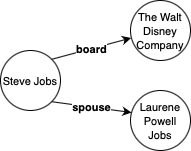
\includegraphics[width=7cm, height=4cm]{chapters/figures/SJ.png}
    \caption{An example knowledge graph}
    \label{fig:kgexample}
\end{figure}

A novice user needs to acquire both knowledge about the underlying ontology structure and proficiency in formulating formal queries (e.g., SPARQL queries) to retrieve information from Linked Data sources. To express the information in terms of SPARQL queries, users have to (a) understand the SPARQL concepts, (b) understand the SPARQL syntax (in absence of a visual query builder) and (c) know what information structures are actually available in order to formulate queries that also return results\cite{sparql}. But this limits the potential of using KGs as information sources to power-users. Therefore, approaches that rely on natural language to describe the information needs of non-expert users have been developed. These systems are called Question Answering (QA) systems.

\section{Question Answering Systems}
Question Answering over knowledge graphs is a difficult and challenging problem that has become popular in recent years. This is mainly due to the intrinsic ambiguity of natural language. Large-scale knowledge graphs such as Wikidata, DBpedia and YAGO have become important resources to solve QA problems. 

For a question answering system to understand a natural language question, it needs to: \begin{enumerate}
\item Identify entities in the question and link them to the corresponding entities in the knowledge graph.  It is a vital
component for a variety of applications built on
knowledge graphs. This involves the two sub-tasks, i.e. Named Entity Recognition (NER) and Disambiguation (NED) tasks. For instance, an ideal NED tool on DBpedia recognizes the entities embedded in the question \textit{"Who is the host of the BBC Wildlife Specials?"} and links them to the corresponding DBpedia entity (e.g., "BBC Wildlife Specials" to
\textbf{BBC\_Wildlife\_Specials}). 

\item Identify relations in the question and map them to the corresponding relations in the knowledge graph. This involves extracting the relations first and then mapping it to the correct relation in the knowledge graph. \textit{Relation Mapping} is about linking surface forms in text representing a relation to equivalent relations (predicates) of a KG\cite{falcon}. In our example question, an ideal relation mapping tool links "host" to \textbf{presenter}.

\item Build a structured representation that connects the entities and relations in the question. Following the step of understanding the question, the question answering system then finds matches between this structured representation and similar structures in the knowledge graph to find answers. 
\end{enumerate}

The focus of this thesis is on \textbf{relation mapping} because it is the most challenging out of the three steps. There has been a lot of work in the literature on entity recognition \cite{chen_shen_huang_wang_2021, OpenTapioca, Weichselbraun, tagme} in comparison with relation mapping. This has been evident if we compare the quality of recent state-of-the-art approaches \cite{falcon2, falcon}. The third step - formulating queries, depends heavily on the previous two steps and usually yields good results if the quality of the output of the first two steps (entity linking and relation mapping) is good. A system that strikes a balance between completely automatic approaches and writing complex queries is an interactive one. Therefore, there is a demand for flexible and collaborative systems to understand users and how systems can be designed to support their tasks. Interactive systems are capable of easing the understanding of a complex system and can be projected and used by inexperienced users across various domains. 

\section{Challenges in Relation Mapping}
Relation mapping faces the following challenges:  
\begin{enumerate}                                               
\item A root word can be represented in multiple ways in a KG making relation mapping difficult. Consider the question, \textbf{Who created Batman?}, the expected relation is \textbf{creator}. Both \textit{created} and \textit{creator} are derived from the root word \textbf{create}.
\item There is a comprehensive lexical gap between the words in the question and how they are represented in the KG, which makes relation mapping challenging. For example, the question \textbf{Who was the first to climb Mount Everest?} does not explicitly mention any reference to the relation \textbf{firstAscentPerson} which is the required relation to form the SPARQL query that can retrieve the answer. 
\item  Some questions need multiple relations to be linked to the target entities to get the correct answer. For instance, \textbf{Give me all cars that are produced in Germany.}, has a SPARQL query as follows,

\begin{quote}
{\fontfamily{qcs}\selectfont SELECT DISTINCT ?uri WHERE \{}
\begin{quote}
\setstretch{1.25}
{\fontfamily{qcs}\selectfont
?uri rdf\footnote{rdf is the prefix of http://www.w3.org/1999/02/22-rdf-syntax-ns\#/}:type \textbf{dbo:Automobile}. \\ \{?uri \textbf{dbo:assembly} res:Germany.\} UNION  \\ \{?uri \textbf{dbp\footnote{dbp is the prefix of http://dbpedia.org/property/}:assembly} res:Germany.\} UNION \\ \{\{?uri \textbf{dbo:manufacturer} ?x.\} UNION \\ \{?uri \textbf{dbp:manufacturer} ?x.\} \\ \{?x \textbf{dbo:locationCountry} res:Germany.\} UNION \\ \{?x \textbf{dbo:location} res:Germany.\}
} 
\end{quote}
{\fontfamily{qcs}\selectfont\}\}}
\end{quote}

This query links to the following relations \textbf{dbo:Automobile, dbo:assembly, dbp:assembly, dbo:manufacturer, dbp:manufacturer, dbo:locationCountry and dbo:location}. The SPARQL query also considers \textbf{dbo:} and \textbf{dbp:} as separate prefixes for relations. In order to get the correct answer, the user needs to know all the above relations to construct a valid SPARQL query.
\end{enumerate}

Several relation mapping tools differ based on the composition of the dataset, the training data, and the complexity of the questions \cite{4}. Most tools are geared towards string similarity and word embedding techniques. In string matching-based similarity analysis, two major similarity indexes are encountered: syntactic similarity and semantic similarity. The syntactic similarity is based on the idea that the degree of similarity between the two texts is proportional to the number of identical words in them. On the other hand, semantic similarity focuses on the meaning and interpretation between the two texts. Semantic similarity methods usually give a ranking or percentage of similarity between the texts, rather than a binary decision as similar or not similar \cite{Chandrasekaran_2022}.
For example, consider two sentences \textit{"John and Mary studied English and Science."} and \textit{"John studied English and Mary studied Science."}. Though these two sentences share the same words they do not convey the same meaning. Similarly, the questions \textit{"How old are you?"} and \textit{"What is your age?"} convey the same meaning, however, they do not have the same set of words.
String matching-based algorithms depend on the number of attempts, the number of character comparisons and the running time. These factors are influenced by the type of algorithm, type of data, data size and length of pattern - one or more strings found within a larger string or text \cite{5}. These algorithms fail to capture the semantic similarity of the sentences. Word embedding techniques like Word2Vec\cite{word2vec}, GloVe\cite{glove}, etc., are better at capturing the semantics of the words but fail when out of vocabulary words are used. They tend to be too specific and do not capture the semantics of the relationships between the entities in the knowledge graph accurately. For example, the question \textbf{Who painted The Storm on the Sea of Galilee?}, a word embedding approach would give relations like \textit{paint, painter,} etc., but it would not capture the relation \textbf{artist}.  

Interactive approaches for query formulation like Sapphire \cite{sapphire}, help the users iteratively construct SPARQL queries by providing auto-complete suggestions \textit{based on the queried data}. These systems require users to have a background knowledge of the entities and the relations to formulate queries with the correct data. The quality of the output of such systems relies excessively on the nature of the input data typed by the user. 

In order to overcome the above limitations, we propose an approach ReMLOFT : \textbf{Re}lation \textbf{M}apping Using \textbf{L}arge Corpus \textbf{O}f \textbf{F}ree \textbf{T}ext, that aims to solve the problem of relation mapping by interactively showing the users a list of candidate relations to choose for a subset of keywords in the question. Our approach aims at reducing the uncertainty faced by QA systems in the task of relation mapping. Suggesting a small set of candidate matches to the user helps in identifying the correct matches more accurately, while not overburdening the user with additional efforts or tasks. This approach heavily relies on using evidence from a large corpus of text to find a substantial number of example sentences. These sentences help in finding relations that can be mapped to connected entities in the knowledge graph. ReMLOFT constructs a free-text knowledge graph from Wikipedia, with entities (Wikipedia page titles) as nodes, and instead of depending on existing relations, ReMLOFT uses free-text sentences as edges. For example, a relation \textbf{ontology/spouse} has 53964 entity pairs and a relation \textbf{property/spouse} has 190949 entity pairs. The sentences extracted from these entity pairs give us meaningful evidence to map relations. 

Consider a triple $\textbf{\textless Steve\_Jobs, spouse,  Laurene\_Powell\_Jobs\textgreater}$, from DBpedia. We find a large number of sentences that relate the two entities \textit{
Steve\_Jobs and Laurene\_Powell\_Jobs } from Wikipedia.  Some of the sentences found are:
{\fontfamily{pcr}\selectfont
\begin{enumerate}
    \item In 1989 Jobs first met his future \textit{wife} Laurene Powell when he gave a lecture at the Stanford Graduate School of Business where she was a student.
    \item Jobs is \textit{married} to Laurene Powell Jobs (Abby Brammell) and has accepted Lisa (Annika Bertea) as his daughter (she now lives with them).
    \item On March 18 1991 Otogawa presided over the \textit{marriage} of Steve Jobs and Laurene Powell.
    \item Laurene Powell Jobs \textit{widow} of Steve Jobs was just behind Domingo inheriting a fortune of \$9 billion.
\end{enumerate}
}
From the above example sentences, we can gather that words in a sentence that connect entities, provide contextual knowledge about the relation between the two entities. Words like \textit{wife, marriage, married} and \textit{widow} from the above example can be used as links to the formal relationship in the knowledge graph (spouse).

We motivate our work by the fact that despite the vast popularity of relation mapping, there are limited attempts to interactive relation mapping over knowledge graphs. Most of the interactive approaches exist for query completion or query construction that help users write syntactically and semantically correct SPARQL queries without prior knowledge of the queried datasets\cite{sapphire}. Our approach aims to bridge the gap between the simple but ambiguous natural language approaches, and the difficult relation mapping problem.

\section{Contributions}
The main contributions of the thesis are as follows:
\begin{enumerate}
\item Building an interactive model for relation mapping that aids in querying data from knowledge graphs, where we provide suggested relations for selected keywords in the question for the user to choose from.

\item  Incorporating external evidence from a large corpus of text to support and guide the approaches used in relation mapping.

\item Building a dictionary of the most frequent keywords that define the context of a relation in the knowledge graph without using lexical tools.

\item Evaluating our approach on recent, most challenging benchmarks used for evaluating question answering systems.

\end{enumerate}

Our approach outperforms statistical and embedding-based relation mapping approaches with significant margins. It gives significant results for complex questions with more than one mapped relations. 

\section{Thesis Organization}
The rest of the thesis is structured as follows: Chapter 2 discusses the related work, and Chapter 3 describes our methodology. The experimental evaluation is presented in Chapter 4. The thesis concludes with Chapter 5.
\end{sloppypar}

\chapter{Related Work}
ReMLOFT is built using the insights of traditional knowledge graphs for question answering and existing approaches on relation mapping for natural language questions. This chapter reviews related work on knowledge graphs, questioning answering systems, interactive systems and relation mapping on natural language questions.

\section{Knowledge Graphs}
Knowledge Graphs are the backbone of the next-generation search and help users discover new information quickly and easily. 
At the heart of modern intelligent systems, the knowledge graphs provide an enormous knowledge reserve and support for intelligent information processing. It has been widely used in medicine, recommender systems and marketing and has very large prospects. Knowledge graphs could be cross-domain or domain-specific. 
Knowledge graphs are additionally categorized into three categories, i.e., \textit{common-sense KGs}: that contain knowledge about the everyday world, \textit{factual KGs}: containing knowledge about facts and events, and \textit{domain KGs}: that encode knowledge from a specific area (linguistics, scientific, biomedical, geographical etc.) \cite{TIDDI2022103627}.
Several knowledge graphs have been made available on the Web in recent years. The most adopted KGs in the literature are publicly available or crowdsourced. Some Enterprise Knowledge Graphs (EKGs), knowledge graphs sourced by large corporations, have been created in the latest years – Google’s \footnotemark[\ref{google}] and Facebook’s social Knowledge Graph, Amazon’s and Ebay’s Product Graphs \cite{TIDDI2022103627}. Examples of popular knowledge graphs used in research are WikiData\cite{wikidata}, DBpedia\cite{dbpedia}, YAGO\cite{yago}, WordNet\cite{wordnet}, Freebase\cite{freebase} (discontinued in 2017) and OpenCyc\footnote{http://www.cyc.com/} (discontinued in 2015). 

WikiData is also a free, collaborative, multilingual, structured project built on top of wiki contents including Wikipedia, Wikivoyage, Wiktionary, Wikisource, etc.\footnote{https://www.wikidata.org/}

DBpedia is a knowledge graph that is extracted from structured data in Wikipedia. The main source for this extraction is the key-value pairs in the Wikipedia infoboxes. It contains 228 million entities, 768 classes and 3000 properties of large cross-domain ontology\footnote{\label{dbp}https://www.dbpedia.org}.

YAGO combines Wikidata and schema.org and contains more than 50 million entities and 2 billion facts\footnote{https://yago-knowledge.org}. 
% YAGO is stored in the standard Resource Description Framework - RDF, each of which consists of a subject, a predicate and an object.

WordNet is a curated lexical database of relationships between concepts (hypernyms, pertainyms, meronyms, etc.).

Advanced AI systems are driven by knowledge graphs, which allows single queries to be turned into an ongoing conversation.
This enables a user to communicate with the system while the system keeps track of the context through each phase of the conversation \cite{Industry-Scale}.

\section{Question Answering using Knowledge Graphs}
Question answering over knowledge graphs aims to use facts in the knowledge graph (KG) to answer natural language questions. 
They provide crisp answers to questions by translating them to precise structured queries over the knowledge graph. A major challenge in a QA system is matching the natural language expressions and the complex schema of the knowledge graph. Consider the question, \textit{"Give me all actors who were born in Paris after 1950."}, which invloves concepts such as "actors", "birthDate" and "birthPlace", that are not easy to map to a structured search over the queried dataset (DBpedia), in addition to requiring a conditional comparison of the results. 

Simple QA links entities to a single relation in the KG. Each question
can acquire the answer from a single fact in the knowledge graph.

As a result, existing methods focus on simple questions answerable with one main relation path in the KG and struggle with complex questions that require joining multiple relations. 
% simple question answering
Some QA systems have achieved good performance on simple questions, i.e., those questions which can be answered by linking to at most one relation and at most one entity in the KG. Lukonikov, et al \cite{10.1145/3038912.3052675}, propose an end-to-end neural network approach that generates a solution for simple questions, which requires the retrieval of a single fact to be answered. They build a knowledge graph-independent representation of entities and relations from textual information associated with the entities or relations. They perform a thorough error analysis that mentions the different types of errors in a QA system like \textit{missing candidates, indistinguishability, hard and soft ambiguity, wrong subject and relation detection}.

Huang, et al \cite{10.1145/3289600.3290956} also focus on simple questions, using a Knowledge Embedding-based Question Answering framework where each question is answered by the machine by using a joint distance metric that takes the structures and relations preserved in the knowledge graph embedding spaces. The KG embedding space is a low dimensional vector representation of all the relations and entities in a KG. They use attention-based bidirectional LSTM models to perform the relation
and entity representation learning.

Another method, TransE-QA \cite{10.1145/3390557.3394296}, solves the problem of simple question answering by combining the knowledge graph representation learning algorithm and the question distributed representation method, by providing the existing question and knowledge graph as input for joint training using the deep learning framework of Tensorflow. They perform their evaluation on the FB5M dataset, which is a subset of Freebase. They visualize the process using a web-based system based on the Flask framework.
% complex question answering

Recently, the focus has shifted towards complex questions comprising of multiple entities and relations.
Existing techniques struggle to match the human-level understanding of questions, even in well-researched topics such as general domain factual question answering. When a query becomes complex, the number of candidates grows exponentially with the number of query components and joins. 

TextRay \cite{textray} is a complex question answering system that automatically translates a complex question to the matching query over the knowledge graph using the decompose-execute-join approach. They use a neural network-based semantic matching model that learns to score candidates for partial queries using implicit supervision from question-answer pairs. TextRay works well on complex questions and gives comparable results on simple questions. Abujabal et al. \cite{10.1145/3038912.3052583} proposed an automated template generation model, namely QUINT, for complex question answering that supports two kinds of templates, i.e., query template and question template based on standard dependency parse trees. The candidate queries are ranked using the random forest classifier. Bio-SODA, proposed by Sima et al  \cite{10.1145/3468791.3469119}, uses a generic graph-based approach for translating user questions to a ranked list of SPARQL candidates queries in scientific datasets without the use of any training data. They rank their queries by combining semantic and syntactic similarity along with node centrality in knowledge graphs.

Another approach that can be quickly adapted to new domains is the Frankenstein \cite{frankenstein} framework relying on machine learning techniques for dynamically selecting suitable QA components and composing QA pipelines based on the input question. Frankenstein uses existing components available in the Question Answering research community into a single platform. 

Our approach builds a similar free text graph from Wikipedia as presented in DELFT \cite{delft}. Delft builds a high coverage and dense free-text knowledge graph, using natural language sentences as edges. To answer questions, delft grounds the question into the related subgraph connecting entities with free-text graph edges and then uses a graph neural network to represent, reason, and select the answer using evidence from both free-text and the graph structure.

Recent advances have enabled the discovery of relevant structured sources of knowledge increasingly achievable. Many modern systems take the existing data with a particular structure or schema and re-use it in a different form. These applications start with an understanding of how data will be used and viewed and create mappings between the schema of the knowledge graphs and the target entities. Knowledge graphs incorporate a wealth of sophisticated knowledge about queries and query manipulation. 

Query discovery is achieved using schema mapping. Schema integration techniques focus on creation of the integrated schemas and creation of queries. A common use of mappings is in query reformulation, commonly referred to as data integration, where queries on a target schema are reformulated, using the mappings, into queries on a source schema.  Clio \cite{renne2000,Fagin2009} is a schema mapping framework, that uses a set of value correspondences (or matchings) that describe how to populate a single attribute of the target schema to find the mapping query. Clio simplifies information integration, by providing tools that help users convert data between representations. Clio mappings assume that given two schemas to map data from the first to the second, the first schema is a source schema, and the second as a target schema. Relation mapping to generate sophisticated queries can be considered a similar problem. To answer a NLQ, we construct queries that specifies the required entities and relations.


\section{Interactive Systems}
Despite extensive research, answering questions remains a difficult task. The user needs to have a deep understanding of each of the steps in a question answering pipeline. Building interactive systems give the user the flexibility to choose the correct answers from given suggestions. Most interactive systems exist for query completion or query suggestion techniques. Sapphire \cite{sapphire}, is one such tool, that helps users write syntactically and semantically correct SPARQL queries without prior knowledge of the queried datasets. Sapphire constructs SPARQL queries, and it removes ambiguity by involving the user directly in query composition. The approach provides autocomplete suggestions with a very low response time that guarantees an interactive experience for users. 

SPARKLIS \cite{sparklis}, a Semantic Web tool helps the users explore and query SPARQL endpoints by guiding them in the
interactive building of questions and answers, from simple ones to complex ones. The users do not need to be familiar with the vocabulary and the schema of the KG. This approach combines different search paradigms like Faceted Search, Query Builders and Natural Language Interfaces. 

Lissandrini et al \cite{x2q} proposed a system named X2Q, for exploring huge knowledge graphs that is both interactive and progressive. The user is guided through the exploration process using an example-based method, in which they first provide a group of entities as partial examples of the desired results, and the system gradually recommends reformulation. X2Q uses the example query paradigm and ranking functions to generate results in a flexible and expressive fashion. They incorporate the user's feedback in the ranking scores to filter the irrelevant suggestions.

Users of interactive systems expect these systems to exhibit behaviours that can be characterized as understanding what the user is looking for, what the user has done and what the user knows \cite{10.5555/1641579.1641586}. Interactive systems refine queries based on the user’s feedback. IMPROVE-QA's \cite{10.1145/3357384.3358059} framework returns answers based on a few feedback over the original answers given by the QA systems. It also enhances paraphrasing dictionaries to ensure a continuous-learning capability in improving QA systems to provide better interactivity and online performance.

\section{Relation Mapping}
One of the main challenges of question answering in knowledge graphs is how to identify which relation within a Knowledge Graph matches the keyword found in a Natural Language question. Researchers have addressed this problem using different approaches.

Mulang’ et al, had the first attempt in mapping keywords to relations in KGs using ReMatch \cite{rematch}. Rematch measures the semantic similarity between the keywords and the relations in KGs based on graph distances from Wordnet\cite{wordnet}. 

Several modern approaches perform both entity linking and relation mapping tasks. EARL \cite{earl} uses the Generalised Travelling Salesman problem and connection density-based machine learning approach between entity nodes in KG. Falcon \cite{falcon} performs joint entity and relation mapping of short text, leveraging several fundamental principles of English morphology and utilizing an extended knowledge graph created by merging entities and relations from DBpedia. Falcon 2.0 \cite{falcon2} utilizes the fundamentals of the initial implementations of Falcon over Wikidata. KBPearl \cite{kbpearl} takes an incomplete KG and a large corpus of text as input to populate the KG. It then employs a semantic graph-based approach to utilize the context knowledge of the facts and the side information inferred from the source text in a global coherence and determine the best results by finding the densest subgraph.

Most works on entity and relation linking rely on the global coherence assumption, i.e., entities and relations within the same document are highly correlated with each other. Lin et al, proposed a technique named TENET \cite{tenet}, which relaxes the coherence assumption in the collective entity and relation mapping in an unsupervised manner as a minimum-cost coherence rooted tree cover problem. However, all these works only improve the output of relation mapping techniques. 

In comparison to all the other works in literature, we do not use sophisticated tools or machine learning models for relation mapping. In ReMLOFT, we investigate the method to map the keywords in the question to the information extracted in free-text sentences as indirect relations between entities which ensures the enhancement and population of candidate relations. ReMLOFT uses the context of keywords for finding relations and does not require training data. In addition, ReMLOFT also provides a dictionary with the most frequent keywords that define the context of a relation in the knowledge graph. ReMLOFT also interacts with the user to provide better candidate relations which helps the user identify semantically related relations to build complex SPARQL queries.



\chapter{Using Free-Text Knowledge Graph in Relation Mapping}
\begin{sloppypar}
This chapter will first discuss the preliminaries of the thesis. This will be followed by a discussion of the construction of a free-text knowledge graph and how it is indexed. We will then discuss how we search the free-text KG and process the data to generate a candidate relation list for Relation Mapping. 

\section{Preliminaries}
\textbf{Knowledge Graph:} A knowledge graph is a directed graph G = {V,E,L} consisting of a set of vertices V (including entities/types/literals) and a set of edges E
that are functionally labeled (relations) by L.

\textbf{Resource Description Framework (RDF) Graph:} RDF is a directed graph composed of triple statements. An RDF graph statement is represented by: 1) a node for the subject, 2) an arc that goes from a subject to an object for the relation and 3) a node for the object. Each triple is represented as $<$s, r, o$>$, where s, o $\epsilon$ V , and r is a relation.

\textbf{Free-Text Knowledge Graph:} A free-text knowledge graph is a multigraph, consisting of nodes V and a set of edges E. Such that any pair of nodes can be connected via multiple edges. Each node is represented by an entity and the edges are text from a corpus.  

\textbf{Natural Language Question, Q:} The natural language questions are divided into two categories, i.e., "simple" and "complex". A simple question is a question that just contains one fact. A complex question contains more than one fact, where the fact is a triple that is not equipped with the relation "type". For instance, the question "\textit{Give me all people that were born in Vienna and died in Berlin.}" is a complex question since it contains two facts, i.e., $<$?e, birthPlace, Vienna$>$, and $<$?e, deathPlace, Berlin$>$.

\textbf{SPARQL Query:} A SPARQL query is a standard query language to retreive and manipulate RDF data. Most cross-domain knowledge graphs such as DBpedia, YAGO, Wikidata, etc., store information in the RDF format. For instance, A SPARQL query that models the question, "Who designed Brooklyn Bridge?", is as follows:
\begin{quote}
{\fontfamily{qcs}\selectfont
% PREFIX res: $<$http://dbpedia.org/resource/$>$ \\
% PREFIX dbo: $<$http://dbpedia.org/ontology/$>$ \\
SELECT DISTINCT ?uri WHERE \{ \\
res:Brooklyn\_Bridge dbo:architect ?uri .\}}
\end{quote}

\section{Free-Text Knowledge Graph}
The Free-Text knowledge graph uses an identical structure as traditional knowledge graphs with nodes (V) and edges (E). They use similar nodes as existing knowledge graphs, where each node represents an entity. The Edges, instead of closed-form relations, are extracted natural language sentences from a corpus \cite{delft}. We use the sentences from the articles in Wikipedia to construct the free-text KG in our approach.

\textbf{Entity Nodes:} The graph inherits Wikipedia entities as the entity nodes.

\textbf{Free-Text Edges:} The Free-Text Edges between nodes are sentences that co-occur in Wikipedia for a pair of entities.

\begin{figure}
\centering
  \begin{minipage}[b]{0.7\textwidth}
    \fbox{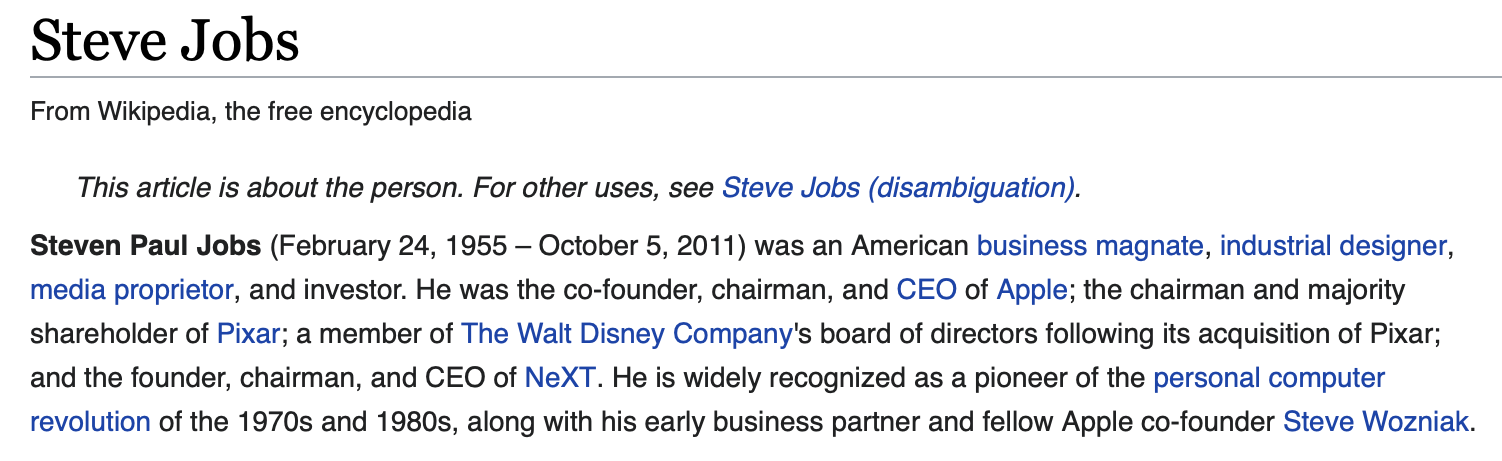
\includegraphics[width=\textwidth]{chapters/figures/SJ1.jpg}}
      \caption{A snippet from the Wikipedia article of Steve Jobs}
    \label{fig:wikisj}
  \end{minipage}
  \end{figure}
The Wikipedia article of an entity: \textit{Steve Jobs} comprises sentences that have other entities Figure \ref{fig:wikisj}. Each of these entities is linked to its own Wikipedia page. Given a sentence from the Wikipedia page of \textbf{Steve Jobs} (E1), {\fontfamily{pcr}\selectfont "the chairman and majority shareholder of \textbf{PIXAR}} (E2)". Both E1 and E2 have their respective Wikipedia pages, but that does not give us enough information to find where the entities appear together.

From the free-text KG we extract: (1) the sentences in E1’s Wikipedia page that mention E2, (2) the sentences in E2’s page that mention E1, and (3) the sentences (anywhere) that mention both E1 and E2 \cite{delft}. Figure \ref{fig:ftkg} shows a snippet from the constructed Free-Text Knowledge Graph.

\begin{figure}
    \centering
  \begin{minipage}[b]{0.7\textwidth}
    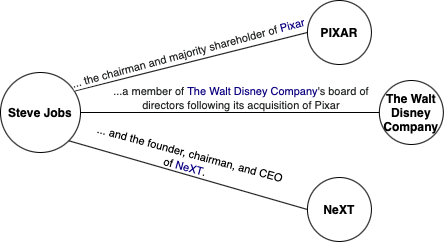
\includegraphics[width=10cm]{chapters/figures/KG1.jpg}
    \caption{A visual example of a Free-Text knowledge graph}
    \label{fig:ftkg}
    \end{minipage}
\end{figure}

\section{Indexing Free-Text KG}
Indexing is used to retrieve data from the database efficiently. Large data-dumps like Wikipedia have several lines of information mapped to various entities. Wikipedia has grown into one of the dominant knowledge sources of mankind, maintained by thousands of contributors \cite{dbpedia}. Indexing helps in querying the free-text knowledge graph to fetch the required results.
The indexed free-text KG has the following information:
\begin{itemize}
    \item \textbf{Page\_id}: An integer, the id of the Wikipedia page.
    \item \textbf{Title}: A string, the title of the Wikipedia page, usually an entity.
    \item \textbf{Text}: A string, sentence in the article that could have more than one entities.
    \item \textbf{Anchored\_Node}: The linked entities in the text. Linked entities refer to entities that have their own pages in Wikipedia. Every anchored\_node is represented as a key-value pair, where the key is the Wikipedia title of the anchored\_node and the value is the \textit{surface form} (the word as it appears in the text), of the anchored\_node. Consider the example sentence in the Wikipedia article of Steve Jobs, "\textit{In 2001, the original \textbf{Mac OS} was replaced with the completely new Mac OS X}". The entity \textit{Mac OS} is an anchored\_node which is represented as ["Classic Mac OS","Mac OS"]. The entity has its own Wikipedia article: \textit{Classic Mac OS} and occurs as \textit{Mac OS} in the Wikipedia article of Steve Jobs.
\end{itemize}
\begin{figure}
    \centering
    % \begin{minipage}[b]{0.7\textwidth}
    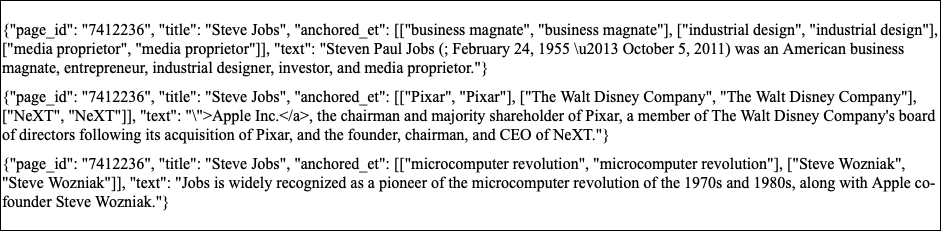
\includegraphics[width=0.8\textwidth,height=3cm]{chapters/figures/SJ2.jpg}
      \caption{Example sentences from the Free-Text Knowledge Graph}
    \label{fig:ftkgsent}
%   \end{minipage}
\end{figure}
Figure \ref{fig:ftkgsent} shows an indexed free text knowledge graph for a snippet of the Wikipedia page of Steve Jobs.

% \subsection{Searching the free-text KG}
The indexed free-text knowledge graph that is constructed has {\fontfamily{pcr}\selectfont 48,977,209} entries. Extracting information from this KG is an extensive task. We use Apache Solr\footnote{\label{solr}https://solr.apache.org/}, a highly scalable, robust, fault-tolerant open-source search platform, that enables easy integration with various programming languages \cite{solr}. Solr search \cite{lucene} manages to search through the index
based on the search string and returns relevant results. When a term is searched, the request handler is processed and then assigned to the query parser accordingly. The query parser validates the query for errors and then transforms it into an Apache Lucene’s Query\footnote{https://lucene.apache.org/core/} format based on the fields. Solr proved effective in our approach for fast retrieval of data due to its ability to achieve fast search responses as it searches using the index instead of the text. In Solr, a Document is the unit of search and index. An index contains one or more Documents, and a Document consists of one or more Fields. The documents of our data comprise of the \textbf{\textit{page\_id, title, anchored\_node}} and \textit{\textbf{text}} as the fields.

\textbf{Extended Knowledge Graph}: DBpedia is one of the most extensive knowledge graphs used in many Question Answering problems. Researchers prefer using DBpedia as it 
i) contains factual data from articles and infoboxes of the English Wikipedia Language Edition (WPLE), ii) is enriched with labels and abstracts from the largest Wikipedia Language Editions, iii) is enriched with links to external knowledge graphs and Web pages, iv) has a rich variety of classes of entities, v) contains approx. 900 million triples (Jan 2021) and is steadily growing. In the last three years, infoboxes in all WPLEs grew by 150\% and the English WPLE doubled in size. We use the DBpedia knowledge graph as it covers many domains\cite{dbpedia}. The DBpedia KG contains over 5.6 million entities and 111 million facts (consisting of subject-relation-object triples), which require over 14.2GB of storage space \cite{dbpedia}. Therefore, we sliced DBpedia and extracted all the relations and their corresponding subject-object pairs to create an extended KG. We boosted our indexed free-text KG with the information from the extended KG. These two separate KGs are used as the principal source of knowledge and act as the core of ReMLOFT.

\textbf{Relations from DBpedia}: \label{sec:relationsfromdbpedia} The relations from DBpedia were extracted from the latest DBpedia dump\footnote{https://www.dbpedia.org/resources/latest-core/}. The DBpedia dump consists of RDF triples represented as (subject,relation,object). Algorithm \ref{alg:sopextract}  explains the extraction of relations from the DBpedia dump.
We create a list of relations \textbf{R} which appends every unique relation encountered in the DBpedia triples (line 5).

\begin{singlespace}
\begin{algorithm}
\caption{Extracting subject,relation,object from DBpedia dump}\label{alg:sopextract}
 \hspace*{\algorithmicindent} \textbf{input}: Triples in the DBpedia dump, $<s,r,o>$ \\
 \hspace*{\algorithmicindent} \textbf{output}:  A hashmap whose key is a relation and value is a list of subject and object pairs, RMap
\begin{algorithmic}[1]
\State \textbf{R} = \{\}
\State RMap = hashmap $<$relation, list$<$(subject, object)$>>$
\For {\textbf{each} t in DBpedia triple }
\If {$t.r \notin \textbf{R}$}
    \State 	\textbf{R} = \textbf{R} $\cup$ t.r
    \State 	RMap[r] = {(t.s, t.o)}
\Else
\State 	RMap[r].add((t.s, t.o))
\EndIf
% \For {\textbf{each} t in DBpedia triple }
%     \State $\mathcal{R}_{DB}$ = $\mathcal{R}_{DB}$ $\cup$ r
%     \State $SO_{r}$= list(s,o)
\EndFor \\
\Return RMap
\end{algorithmic}
\end{algorithm}
\end{singlespace}

We only considered the relations that were of the  ontology/ (dbo:) or property/ (dbp:) types. Table \ref{tab:countrelations} shows the number of relations extracted from the DBpedia dump.
\begin{table}[H]
    \centering
    \begin{tabular}{|c|c|}
     \hline
     \textbf{Relations from DBpedia} & \textbf{Count} \\
    \hline
     ontology/ & 1437 \\
    \hline
    property/ & 52477 \\
    \hline
    \textbf{Total} & \textbf{53914} \\
    \hline
    \end{tabular}
    \caption{Number of relations in DBpedia}
    \label{tab:countrelations}
\end{table}

Some of the observations on the relations extracted from DBpedia's latest core that makes relation mapping more challenging are as follows:

\begin{enumerate}
\item Many relations occur in both the dbo: and dbp: namespace (850 relations). For example, \textit{dbo:spouse and dbp:spouse} are both valid relations in DBpedia. 

\item The DBpedia dump has relations with numerous spelling and captilization errors : \textit{dbp:date, dbp:Date, dbp:dAte, dbp:daTe, dbp:datE}, but they are considered as a single end url point in DBpedia.

\item Relations can be singular or plural. For instance, \textit{dbp:spouse, dbp:spouses}.

\item  The relations have special characters: punctuation marks (\textit{dbp:nextYear'sRace}), numbers (\textit{dbp:firstRider125Bike}), Greek Letters and characters from other languages apart from English.

% \item The dbp: or dbo: values could reference an rdf:type. RDF types are  used to state that an entity is an instance of a class. They do not define a relation, instead they point to an entity in DBpedia. For a natural language statement, \textit{"Proinsulin a protein"}, the triple is represented as 
% $<$Proinsulin,rdf:type,dbo:Protein$>$, 

\item Relations are concatenated strings in Camel case. For example, \textit{dbp:militaryRank and dbo:significantBuilding}.
\end{enumerate}

Hence, we filtered these relations by removing punctuation marks, Greek Letters, characters from other languages to make our process efficient. For relations that occur in both the dbo: and dbp: namespace, we consider them as one relation. For instance \textit{dbo:spouse} and \textit{dbp:spouse} is considered as one relation \textit{spouse}. We will refer to this list of filtered relations as $\mathcal{R}_{DB}$. $\mathcal{R}_{DB}$ represents the pool of all relations that make up our search space for the task of relation mapping.

\textbf{Subject-Object pairs from DBpedia}: Entities in DBpedia are connected by one or more relations. The entities are referred to as the subjects or objects connected using a relation. For every relation in \textbf{R} we can have various subject-object pairs. t.s, t.r and t.o represents the subject, relation and object in the DBpedia triple, respectively. We create a hashmap called RMap, whose key is the relation in the triple and value is a list of subject- object pairs. For every triple in DBpedia the list of subject-object pairs are extracted along with the relation. If a relation is unique, a new key is generated in RMap, otherwise, the subject-object pair is added to the list of the existing relation.
Figure \ref{fig:subject-object} shows a snapshot of some of the subject-object pairs for a relation dbo:largestCity, where the object (right) represent the largest city in the subject (left). The relation \textbf{dbo:largestCity} has 3247 subject-object pairs and \textbf{dbp:spouse} has 963 subject-object pairs.

\begin{figure}
    \centering
   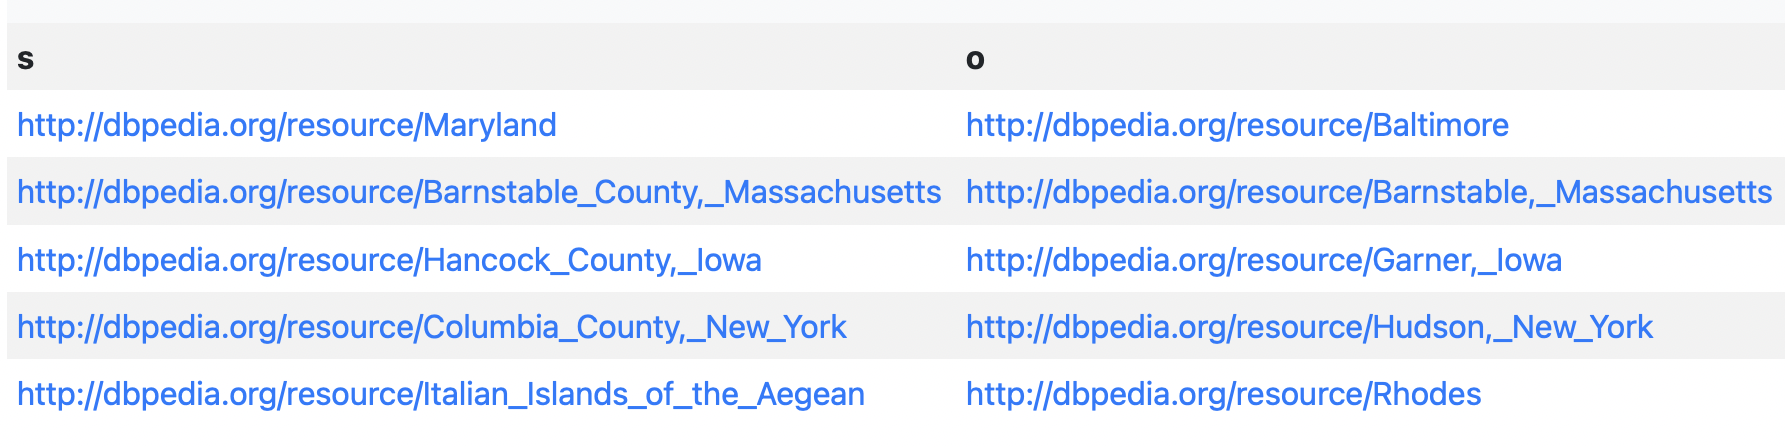
\includegraphics[width=15cm, height=4cm]{chapters/figures/subject-object.png}
    \caption{Snapshot of Subject-Object pairs for dbo:largestCity}
    \label{fig:subject-object}
\end{figure}

\subsection{Sentence Extraction}
Each relation in $\mathcal{R}_{DB}$ has numerous subject-object pairs. These subject-object pairs (anchored\_nodes) co-occur in sentences in the text corpus that we used, and are therefore stored in our free-text KG. Other approaches use linguistic resources such as Oxford dictionary\footnote{Oxford English Dictionary. 2nd ed. Oxford: Oxford University Press, 2004}, and semantic dictionaries like WordNet\cite{wordnet} to provide
synonyms, derived word forms, etc. The sentences extracted are a wealth of information as they contain the entities, their context and other lingual facts. We extract these shared sentences and utilize this information to extract words for relation labels.
\begin{singlespace}
\begin{algorithm}
\caption{Extracting sentences from FTKG}\label{alg:sentextract}
 \hspace*{\algorithmicindent} \textbf{input}: RMap, $\mathcal{R}_{DB}$ \\
 \hspace*{\algorithmicindent} \textbf{output}:  A hashmap whose key is a relation and value is the sentences retreived from FTKG, SMap
\begin{algorithmic}[1]
\State SMap = hashmap$<$relation, list$<$sentence$>>$
\For {\textbf{each} r in $\mathcal{R}_{DB}$}
\For {\textbf{each} (s,o) in RMap[r]}
    \State SMap[r].add(SELECT text from FTKG where s and o in title, anchored\_node, text)
\EndFor 
\EndFor \\
\Return SMap
\end{algorithmic}
\end{algorithm}
\end{singlespace}
Algorithm \ref{alg:sentextract} explains the process of extracting sentences for every relation r in $\mathcal{R}_{DB}$. The input to this algorithm is the hashmap RMap, which has the key as the relations and value as the list of subject-object pairs, obtained in Algorithm \ref{alg:sopextract} and the list of filtered relations $\mathcal{R}_{DB}$.
Each (s,o) pair in RMap is searched in the indexed free-text KG using Solr. Solr searches for the s and o in the title, anchored\_node and text fields of the free-text KG. The \textit{text} that contains both the s and o are added to SMap (line 4). 
The output of this algorithm is SMap which is a hashmap whose key is the relation and the value is the sentences obtained from the free-text KG for the subject-object pairs of that relation. 

A sample Solr query that searches the subject-object pair: Steve Jobs, Laurene Powell Jobs is as follows:
\begin{quote}
{\fontfamily{qcs}\selectfont select?fl=text\&q= \\
(text:"Steve Jobs" AND text:"Laurene Powell Jobs") OR \\
(title: "Steve Jobs" AND title:"Laurene Powell Jobs" ) OR \\
(anchored\_node:"Steve Jobs" AND anchored\_node:"Laurene Powell Jobs")}
\end{quote}
Here, fl represents the field \textit{text} to be returned and q represents the \textit{search entity} which is the subject and the object. 

The output of this algorithm is a hashmap whose key is the relation r, and value is a list of sentences represented by SMap. For each relation in $\mathcal{R}_{DB}$, we store the sentences that are extracted from the indexed free-text knowledge graph.

\subsection{Text Cleaning Pipeline}
\label{sec:TextCleaningPipeline}
Text Cleaning Pipeline comprises of a series of modules which is used to clean the sentences connecting the relation to its subject-object pairs.
Algorithm \ref{alg:dictcreation} shows how the extracted sentences in SMap (output of Algorithm \ref{alg:sentextract}) is used to create a dictionary of words for each relation in $\mathcal{R}_{DB}$. Figure \ref{fig:graphConstruct} explains the approach for an example relation \textbf{spouse}. 

\begin{singlespace}
\begin{algorithm}
 \hspace*{\algorithmicindent} \textbf{input}: SMap, $\mathcal{R}_{DB}$  \\
 \hspace*{\algorithmicindent} \textbf{output}: A hashmap of whose key is a relation and value is a list of (keyword, frequency) pairs, Dict
\begin{algorithmic}[1]
\caption{Text Cleaning Pipeline}\label{alg:dictcreation}
\State Dict = hashmap$<$relation, list$<$(keyword, frequency)$>>$
\For {each r in $\mathcal{R}_{DB}$}
\For {each s in SMap[r]}
    \State Text-Preprocessing(s) //Removes punctuation, links and numbers
    \State Tokenization and Stopword Removal(s) //splits the sentence into tokens and removes stopwords
    \State Lemmatization(s) //converts the tokens into lemma
    \State $List_{r}$ = clean keywords in s
    \State UpdateCount(Dict[r], $List_{r}$)
\EndFor
\EndFor
\State \textbf{return} Dict
\end{algorithmic}
\end{algorithm}
\end{singlespace}

\textbf{Text Pre-processing}: Text pre-processing plays a vital role in text mining. The first module under the Text Cleaning Pipeline is illustrated in Figure \ref{fig:graphConstruct}. This module removes the input text's links, HTML tags, numbers, and punctuation as these tokens do not add valuable information to our text (line 4). 

\textbf{Tokenization and Stopword Removal}: The next module creates tokens from the output of the Text Pre-processing module. 
We use the word\_tokenize() function from the NLTK\footnote{{\label{nltk}}https://www.nltk.org} library to break the sentences into possible tokens. The NLTK library also has a corpus of stopwords in various languages. The most common words in Wikipedia articles are pronouns, prepositions, articles etc., such as \textit{a, the, who, is, on, etc}. These words have negligible lexical content. 
We use the English language corpus to remove stopwords from these sentences. Removing stopwords reduces the extent of term space by reducing the total number of terms in the system, and hence, reducing the size and complexity of the system. Stopwords are removed from documents because those words are not considered as keywords in text mining applications\cite{porter_1980}.

\textbf{Lemmatization}: The final module in the Text Cleaning Pipeline converts the tokens to their lemmas (line 6). The lemma is the base form of the token. They can be obtained using rules based on part-of-speech tags, or lookup tables.\cite{spacy}. Modern lemmatization algorithms in comparison with stemming, provide higher quality lemmas\cite{9467919}. SpaCy is the current state-of-the-art technique that processes and interprets large volumes of text. Lemmatization using the SpaCy library as compared to NLTK\footnotemark[\ref{nltk}] is the most effective according to the quality criterion as they include the processing of endings such as \textit{-ed, - ing}, regardless of the publication topic\cite{9467919}. The recent upgrade of spaCy is more effective in POS (parts-of-speech) tags than their previous versions\cite{spacy}. 

For example, if the input text to the Text Cleaning Pipeline is, "{\fontfamily{pcr}\selectfont The first generation of iPod was released October 23, 2001.}", the output of the lemmatization module would be a list of five keywords {\fontfamily{pcr}\selectfont ["first", "generation", "ipod", "release", "october"]}.

\begin{figure}
    \centering
    \fbox{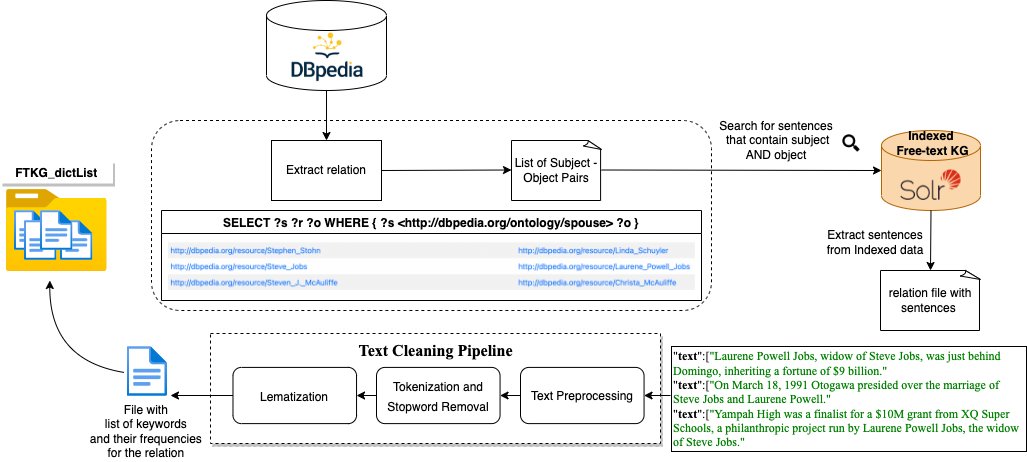
\includegraphics[width=15cm, height=7cm]{chapters/figures/GraphConstruct.png}}
    \caption{Dictionary Construction}
    \label{fig:graphConstruct}
\end{figure}

\textbf{Dictionary Creation}: The output of the Text Cleaning Pipeline is a list of keywords from the sentences in SMap (line 7). A dictionary is created from this list of keywords. We use a counter to tally the frequency of keyword occurrence in the file (line 8). The higher the count, more the keyword relates to the relation. We filter the top 100 keywords in each of these relation files. 

The total number of unique keywords obtained for each relation varies greatly. Some relations have keywords with a frequency of 100,000 while some relations have keywords with a frequency of 1. Relations that have keywords with frequencies in the order of thousands have a large number of unique keywords ($\sim$ 100 thousand words). In order to obtain a consistent parameter across all the relations with varying frequencies of occurrence, we choose the top 100 keywords. We found that the top 100 keywords contribute to the most associated words for a given relation as compared to using all the words in the relation files.

The output of Algorithm \ref{alg:dictcreation} is the dictionary Dict, which is also a hashmap whose key is the relation and value is a list of 100 keywords-number of occurrences pairs.

Using the example relation \textbf{spouse}, the top 3 keywords in the dictionary for \textbf{spouse}, Dict[spouse], are {\fontfamily{pcr}\selectfont
("marry", 93733), ("wife", 47744), ("daughter", 34588)
}.
\section{Using the Free-text KG}
{\label{usingfreetextkg}}
The relation list with the most common words along with their frequency of occurrence formulated from free-text KG, is the foundation knowledge graph of ReMLOFT, \textbf{Dict}. We will use the following question as a running example throughout this section, Q: {\fontfamily{pcr}\selectfont Which river does the Brooklyn Bridge cross?}.

\subsection{Pre-processing the Natural Language Question}
\label{sec:preprocessnlq}
The objective of this pre-processing is to extract the candidate keywords in the question that can be used to map to relations in the KG. This pre-processing includes (1) identifying entities in the question, (2) removing these entities, and (3) preparing the remaining keywords.

\textbf{Identifying Entities:} We first identify the entities in the question Q as the Question Entity Nodes, $E_{Q}=\{e_{i} | e_{i} \in Q \}$.  In Figure \ref{fig:approach}, the entity in the Question is \textbf{Brooklyn Bridge}. For a question with multiple entities: {\fontfamily{pcr}\selectfont In which films directed by Garry Marshall was Julia Roberts starring?}, the system identifies \textbf{Gary Marshall} and \textbf{Julia Roberts} as the entities. Several NER approaches can be used to identify the entities in the question \cite{falcon, falcon2}. 

\textbf{Removing Entities:} Once identified, the entities $E_{Q}$ are removed from the question. If the entity is a n-gram (n words), all the words occurring in the entity are removed from the question. In our example question, \textit{Brooklyn\_Bridge} is a bi-gram entity found in DBpedia, hence, the keywords Brooklyn and Bridge are removed from the question.

\begin{figure}[h]
    \centering
   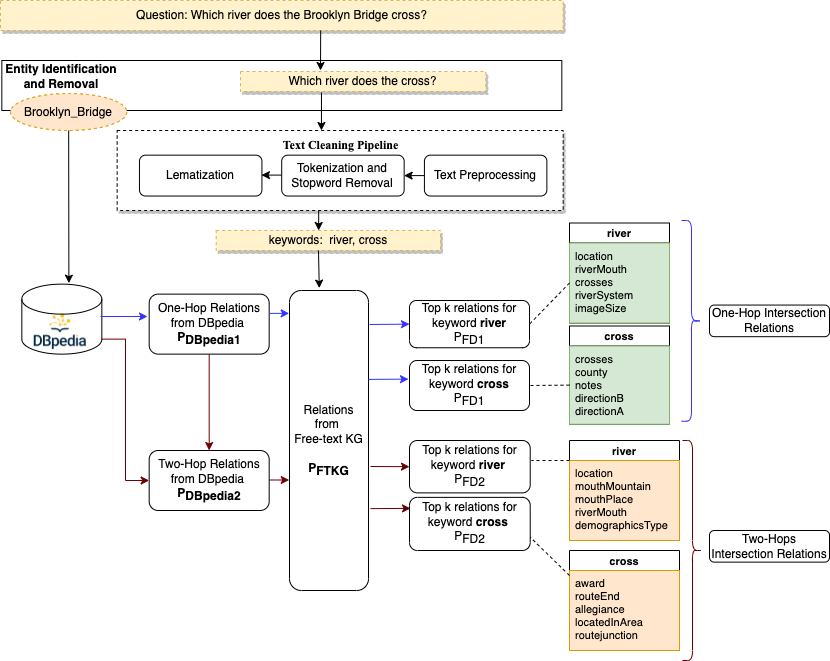
\includegraphics[width=15cm, height=10cm]{chapters/figures/Approach.png}
    \caption{Illustration of the steps of ReMLOFT using the example question "Which river does the Brooklyn Bridge cross?"}
    \label{fig:approach}
\end{figure}

\textbf{Preparing Remaining Keywords:} Once the entities $E_{Q}$ are removed from Q, the other keywords in Q are passed through the modules of the Text Cleaning Pipeline to obtain the lemmatized Keywords, $KW_{Q}=\{kw_{i} \; |\; kw_{i} \in Q \}$. The keywords first undergo Text pre-processing, where the punctuation, numbers and links are removed. They are then tokenized followed by the removal of stopwords. Finally, the keywords are lemmatized to their lemma which is the base form of the keyword. In our running example question, after the removal of the entities, \textit{"Which river does the cross?"}, are the remaining keywords in the question. After the processing the keywords, we get \textit{river} and \textit{cross} as the final keywords that we will use for relation mapping.

\subsection{Extracting candidate relations from DBpedia}
The objective of this step is to reduce the search space of relations from which we will map tokens in the questions to the relations. We do this by focusing on the set of entities $E_{Q}$ extracted from Q. These entities are queried in DBpedia to retrieve the relations associated with them. Algorithm \ref{alg:candidaterelations} shows the extraction of candidate relations from DBpedia. The input of Algorithm \ref{alg:candidaterelations} is the set of entities $E_{Q}$ extracted from Q. The output is a list of relations found one-hop or two-hops away from the entities in $E_{Q}$.

\begin{singlespace}
\begin{algorithm}
\caption{Extracting candidate relations from DBpedia}\label{alg:candidaterelations}
 \hspace*{\algorithmicindent} \textbf{input}: Entities from the Question, $E_{Q}$   \\
 \hspace*{\algorithmicindent} \textbf{output}: A list of candidate relations at one-hop and two-hops intersection
\begin{algorithmic}[1]
\For {\textbf{each} e in $E_{Q}$}
    \State $P_{DBpedia1}$= SELECT distinct ?r where \{?e ?r ?o UNION ?s ?r ?e\}
        \State Pre-process $P_{DBpedia1}$
    \For {\textbf{each} r in $P_{DBpedia1}$}
        \State $P_{DBpedia2}$=
        \State SELECT DISTINCT ?r where
        \State\{e ?r ?x. \{?x ?r ?o.\} UNION \{?s ?r ?x.\}\} AND 
        \State SELECT DISTINCT ?r where 
        \State \{?x r e.\{?x ?r ?o.\} UNION \{?s ?r ?x.\}\}
    \EndFor
    \State Filter unique /ontology \& /property relations
\EndFor
% \State $P_{DB}=P_{DBpedia1} \cup P_{DBpedia2}$
% \State \textbf{return} $P_{DB}, P_{DBpedia1}, P_{DBpedia2}$
\State \textbf{return} $P_{DBpedia1}, P_{DBpedia2}$
\end{algorithmic}
\end{algorithm}
\end{singlespace}


\textbf{First-Hop relations} $P_{DBpedia1}$: The relations that link an entity to its nearest neighbour (line 2). A given entity can be a subject or an object when connected using a relation. We find all the distinct relations that connect the entity to another entity in DBpedia.

\textbf{Second-Hop relations} $P_{DBpedia2}$: The relations that link the nearest neighbour to their neighbours (second-hop neighbour) (lines 5-9). 

\begin{figure}
    \centering
   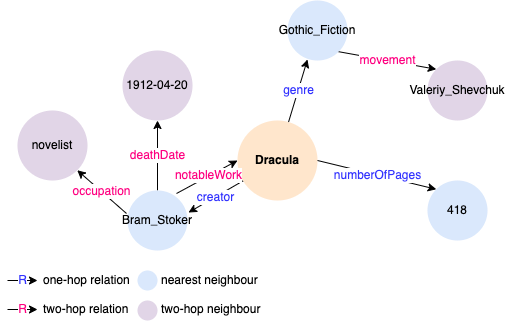
\includegraphics[width=12cm, height=8cm]{chapters/figures/Hop.png}
    \caption{The one-hop and two-hops relations and entities for dbr:Dracula}
    \label{fig:hop}
\end{figure}

We use the concept of two hops as some questions have answers in the second hop relations. While questions like our running example have the correct answer as one of the one-hop neighbouring entities, questions like {\fontfamily{pcr}\selectfont When did the creator of Dracula die?}, whose subgraph is shown in Figure \ref{fig:hop}, have the correct answer as one of the second-hop neighbouring entities. In the above example, the question has two keywords \textbf{creator} and \textbf{die} that should be mapped to the relations \textbf{creator} and \textbf{deathDate}, respectively. The relation \textbf{creator} is obtained one hop away from the entity, \textbf{Dracula}, identified in the question. However, the second relation \textbf{deathDate} is two-hops away from \textit{Dracula}. In order to retrieve \textbf{deathDate} we first traverse to the creator \textbf{Bram\_Stroker} and then to the deathDate of Bram\_Stroker, \textbf{1912-04-20}. 

We limit our approach to the second hop relations as the number of neighbours increase exponentially with the number of hops.  We use the entities as both the subject and the object while querying in Dbpedia, Algorithm 4 (line 6-9). 

Therefore, starting from the identified entities in the questions $E_{Q}$, we retrieve all the one-hop and two-hops away relations $P_{DBpedia1}$ and $P_{DBpedia2}$, respectively.

% A unique list of relations is obtained by combining the one-hop and two-hops away relations, $P_{DB}$ (line 13).
% \begin{equation}
%   P_{DB}=P_{DBpedia1}\cup P_{DBpedia2} 
% \end{equation}

\begin{singlespace}
\begin{algorithm}
 \hspace*{\algorithmicindent} \textbf{input}: Tokenized and Lemmatized keyword: key  \\
 \hspace*{\algorithmicindent} \textbf{output}: List of candidate relations from FTKG, $P_{FTKG}$
\begin{algorithmic}[1]
\caption{Extracting candidate relations from the Free-Text KG}\label{alg:extractFTKG}
\For {key in $KW_{Q}$}
\For {each entry in List(keyword, occurrencesNum)}
        \If {key == keyword}
            \State $P_{FTKG}$ = $P_{FTKG}$ $\cup$ (r,[key,occurencesNum])
        \EndIf
\EndFor
\EndFor
\State \textbf{return} $P_{FTKG}$
\end{algorithmic}
\end{algorithm}
\end{singlespace}

\subsection{Extracting Candidate Relations from the Free-text KG}
\label{sec:extractftkgrelations}
The question after the removal of the entity is left with a string of keywords $KW_{Q}$. For our running example question: the keywords obtained are $KW_{Q}$={\fontfamily{pcr}\selectfont river, cross}. Algorithm \ref{alg:extractFTKG} explains the steps for relation extraction from the Free-Text KG. Every keyword in $KW_{Q}$ (processed keywords) is searched in the all the dictionaries $Dict_{r}$, which is list of keywords and the number of occurrences of the keywords. If the search is successful, the \textit{relation} is concatenated with the keyword and number of occurrences which is represented as \textbf{(relation: [keyword, occurencesNum])} (line 4). The output of this extraction algorithm is a list of relations from the free-text KG, $P_{FTKG}$. We sort this list based on the \textbf{occurencesNum} of the keyword.

\subsection{Candidate List Generation}
\label{sec:candidatelist}
The output of the previous processes are the following sets of relations: 
\begin{enumerate}
    \item $P_{DBpedia1}$ (the one-hop relations from the entities identified in the question),
    \item $P_{DBpedia2}$ (the two-hops relations from the entities identified in the question), 
    \item $P_{FTKG}$ (the relations associated with sentences that include the keywords in the question).
\end{enumerate}
 In this final step, the objective is to generate the top-k candidate relations to display to the users to choose from. This is going to be based on the intersections of the aforementioned sets of relations as follows:

\textbf{One-Hop Intersection Relations, $P_{FD1}$} : This is the intersection of the one-hop relations from DBpedia, $P_{DBpedia1}$ and the relations obtained from the free-text KG, $P_{FTKG}$. This is sorted based on number of occurrences of the keyword in $P_{FTKG}$.
\begin{equation}
    P_{FD1}=P_{DBpedia1} \cap P_{FTKG}
\end{equation} 
% As shown in Figure \ref{fig:my_label}, for k=3, the keyword \textbf{river} matches {\fontfamily{pcr}\selectfont location, riverMouth and crosses} and the relation \textbf{cross} matches {\fontfamily{pcr}\selectfont crosses, country and notes}.
% \[P_{FD1}=P_{DBpedia1} \cap P_{FTKG}\]

\textbf{Two-Hops Intersection Relations, $P_{FD2}$} : This is the intersection of the two-hops relations from DBpedia, $P_{DBpedia2}$ and the relations obtained from the free-text KG, $P_{FTKG}$. This is sorted based on number of occurrences of the keyword in $P_{FTKG}$.
\begin{equation}
    P_{FD2}=P_{DBpedia2} \cap P_{FTKG}
\end{equation} 

% \textbf{Final Intersection, $P_{Final}$} : The relations obtained by combining the relations in the one-hop intersection relations and the two-hops intersection relations.
% \begin{equation}
%     P_{Final}=P_{FD1}+P_{FD2}
% \end{equation}

Figure \ref{fig:approach} shows the one-hop and two-hops intersection relations for our running example question where k=5 , based on the number of occurrences. The keyword \textbf{river} matches {\fontfamily{pcr}\selectfont location, riverMouth, crosses, directionB and directionA} and the relation \textbf{cross} matches {\fontfamily{pcr}\selectfont crosses, country, notes, riverSystem, imageSize} in the one-hop intersection. The keyword \textbf{river} matches {\fontfamily{pcr}\selectfont location, mouthMountain, mouthPlace, riverMouth and demographicsType} and the relation \textbf{cross} matches {\fontfamily{pcr}\selectfont award, routeEnd, allegience, locatedInArea and routeJunction} in the two-hops intersection.

\section{Interactive User Interface} 
We introduce an interactive user interface for ReMLOFT. This interface is shown in Figure \ref{fig:userinterface}. The user interface presents a text box for the user to type their natural language question. After the user clicks "\textbf{Recommended Relations}", the question is pre-processed using the steps discussed in Section \ref{sec:preprocessnlq}. The interface displays the processed keywords and the top-5 candidate relations extracted from the one-hop relations for each displayed keyword. In our running example, the user enters the question and we display the top-5 relations for the keywords \textit{river} and \textit{cross}.

% We propose a modified method where we display the best of the two results obtained from the One-Hop Intersection Relations, $P_{FD1}$ and Two-Hops Intersection Relations, $P_{FD2}$. This is effective for complex questions who have correct answers in the relations that are present two-hops away. 

In case the displayed relations do not satisfy the user's information needs, they can view an extended list pf candidate relations by clicking on "\textbf{View More Relations}". This would display the two-hops intersection relations for each keyword. 
\begin{figure}[h]
    \centering
    \fbox{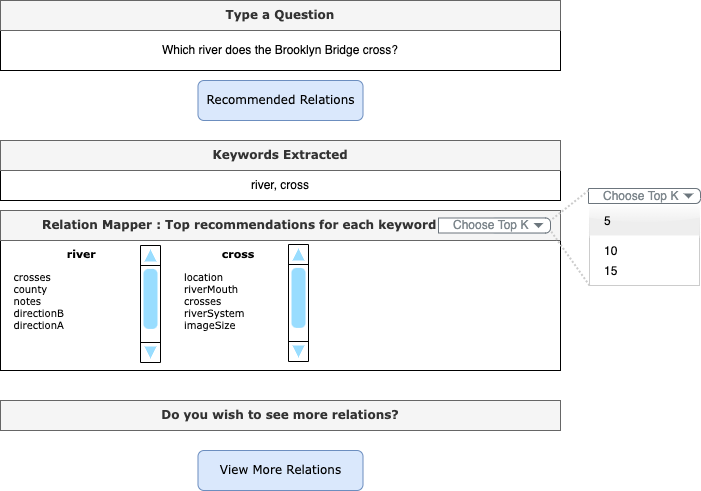
\includegraphics[width=\textwidth, height=11cm]{chapters/figures/interactive-2.png}}
    \caption{User Interface of ReMLOFT}
    \label{fig:userinterface}
\end{figure}
Given the typically large number of candidate relations obtained from the One-Hop Intersection Relations, $P_{FD1}$ and Two-Hops Intersection Relations, $P_{FD2}$ in a dataset, we limit the number of recommendations to top-5. We provide the user the flexibility to restrict or expand the top-k value from a drop-down. The idea is that the system assists the user to enhance query construction. 
The recommended relations help the user build superior SPARQL queries to retrieve answers to their questions over any knowledge graph. 

\end{sloppypar}
\chapter{Experimental Evaluation}
In this chapter, we discuss the datasets, the baselines, the metrics used, the results and the limitations of ReMLOFT. We used the Debian GNU/Linux Machine, with eight cores and 52GB RAM for the implementation of our approach.

\section{Datasets}
We use the Question Answering over Linked Data (QALD) datasets in our evaluation as QALD\footnote{http://qald.aksw.org/} challenge has established itself as a well-known KGQA competition on DBpedia. For each edition of the challenge, new datasets (benchmarks) for training and testing have been published. QALD includes nine benchmarks from QALD-1 to QALD-9. 

Each question in these datasets is accompanied by a SPARQL query that include the gold standard relations. Due to the evolving nature of knowledge graphs and the fact that they are continuously changing, we filtered the questions in these datasets by running the SPARQL queries against DBpedia to check if they indeed return answers. Questions in the QALD datasets vary in complexity and include simple and complex questions. 

We used the following benchmarks in particular: 

\textbf{QALD-5}  \cite{qald5}: This benchmark consists of over 340 training questions and focuses on multilingual question answering. We restrict our work to questions in English. After filtering, we get 206 questions.

\textbf{QALD-7} \cite{qald7}: The training data consists of 215 questions compiled and curated from previous challenges. The questions vary based on their complexity, including questions with counts (e.g., \textit{How many languages are spoken in Colombia?}), superlatives (e.g., \textit{Which Indian company has the most employees?}), comparatives (e.g., \textit{Give me all books by William Goldman with more than 300 pages.}), and temporal aggregators (e.g., \textit{Do Prince Harry and Prince William have the same parents?}). After filtering the queries, we end up with 168 questions.

\textbf{QALD-9} \cite{qald9}: This is the latest benchmark from the QALD challenge and consists of over 408 training questions curated from previous challenges. We get 344 questions after filtering the queries.

\begin{table}[H]
    \centering
    \begin{tabular}{|c|c|c|}
     \hline
    \textbf{Datasets} & \textbf{\#Q} & \textbf{Filtered \#Q} \\ [0.3ex] \hline
    \textbf{ QALD-5} & 340 & 206 \\ 
     \hline
    \textbf{ QALD-7} & 215 & 168 \\
     \hline
    \textbf{ QALD-9} & 408  & 344 \\
     \hline
    \end{tabular}
    \caption{Questions in the QALD Datasets}
    \label{tab:QALDdatasets}
\end{table}

\begin{table}
    \centering
    \begin{tabular}{|c|c|c|c|}
    \hline
    \textbf{\#Relations} & \textbf{QALD-5} & \textbf{QALD-7} & \textbf{QALD-9} \\
    \hline
     No Relation & 7  & 0 & 7\\
     \hline
    1 Relation & 148 & 133 & 257\\ 
     \hline
    2 Relations & 41 & 29 & 61\\
     \hline
    3 Relations & 8  & 6 & 18\\
     \hline
    4 Relations & 2  & 0 & 1\\
     \hline
    \textbf{Total} & \textbf{206}  & \textbf{168} & \textbf{344}\\
     \hline
    \end{tabular}
    \caption{Number of relations in the QALD Datasets}
    \label{tab:QALDrelations}
\end{table}

The number of questions that we use in our evaluation are summarized in Table \ref{tab:QALDdatasets}. Table \ref{tab:QALDrelations} shows the number of viable questions that are grouped into five categories, based on the number of relations in the SPARQL queries associated with the questions in the benchmarks. The \textit{No relations} refers to questions that do not have a relation in the SPARQL query. These questions usually return the rdf:type. For example., \textit{Is Proinsulin a protein?} has a SPARQL query,

{\fontfamily{qcs}\selectfont
\textit{
ASK WHERE \{res:Proinsulin rdf:type dbo:Protein.\} 
}}

We do not consider the rdf:type as relations for our relation mapping approach. Hence, this question is considered as a\textit{ No Relation} question. \textit{1 Relation}, \textit{2 Relations}, \textit{3 Relations} and \textit{4 Relations} are questions with one, two, three and four expected gold standard relations, respectively.

\section{Metrics}
In this section, we consider three evaluation metrics to evaluate our approach.

\subsection{Hits@k}
The relation mapping task is recast as a ranking problem for evaluation, as described in \cite{sun2019pullnet, 10.1145/3437963.3441753}. For each test question in the dataset, a candidate list of relations is returned. We adopt the widely used evaluation metrics in previous works named Hits@k. Hits@k indicates the proportion of correctly aligned relations ranked in the top-k predictions. It represents if the number of gold standard relations in the candidate list occurs in the recommended top-k candidate relations. The value of hits@k ranges between 0 (miss) to 1 (hit). Any value in between denotes partially found relations (for questions that map to multiple relations in the KG).

To evaluate the performance of ReMLOFT and the baseline experimental settings, we employ Hits@5, Hits@10 and Hits@15 . We do not consider Hits@1 as most complex questions have multiple relations to formulate the query.
\begin{equation}
hits@k=\frac{Number \ of \ correct \ relations \ found}{Number \ of \ expected \ relations \ (gold \ standard \ relations)}
\end{equation}

The hits@k for all the questions in the dataset is calculated as:
\begin{equation}
    Hits@k=\frac{\sum_{i=1}^N hits@k_i}{N}
\end{equation}

Where N denotes the number of questions in the dataset and i indicates the question in the dataset.

\subsection{Coverage}
Coverage is defined in \cite{robertsetal}, as the percentage of questions for which at least one correct relation is retrieved. 
\begin{equation}
    Coverage=\frac{\#Questions \ that \ return \ at least \ one \ correct \ answer}{N} * 100
\end{equation}
Where, N denotes the number of questions in the dataset.
 In a QA context, global measures such as precision and recall are not as helpful as coverage \cite{robertsetal}.

\subsection{Accuracy}
Accuracy is defined by the ratio of the correctly identified relations over the total number of relations present in a dataset. This metric has been used for evaluation in popular Question Answering systems like EARL \cite{earl}.
\begin{equation}
    Accuracy=\frac{ Total \ Relations \ returned}{M} * 100
\end{equation}
Where, M denotes the number of relations in all the questions in the dataset.

\section{Baselines}
\label{sec:baselines}
We compare our approach against three popular baselines used in natural language processing of question answering systems.

\subsection{String Similarity} 
\label{sec:stringsimilarity}
We analyzed two string similarity techniques on the Free-Text Knowledge graph.

\textbf{Levenshtein distance.} 
Levenshtein distance is used to calculate the proximity of match, which is the number of primitive operations - addition, deletion and substitution, necessary to translate the string into an accurate match. A lower distance implies greater similarity between the two strings.
Mathematically, the Levenshtein distance \footnote{https://en.wikipedia.org/wiki/Levenshtein\_distance\#} between two strings a and b, of length $|a| \ and \ |b|$, respectively, is given by 

\begin{singlespace}
\begin{equation}
lev(a,b) = \left\{ \begin{array}{cl}
|a| & if \ |b|=0, \\
|b| & if \ |a|=0, \\
lev(tail(a),tail(b)) & if \ a[0]=b[0], \\
1 + min = \left\{ \begin{array}{cl}
lev(tail(a),b) \\
lev(tail(a),tail(b)) \\
lev(a,tail(b))\\
\end{array} \right.& otherwise,
\end{array} \right.
\end{equation}
\end{singlespace}

where, the \textit{tail(x)} of the string x is a string of all but the first character of x. For example, \textit{tail(rain)} denotes \textit{"ain"}. The first element in the minimum \textit{lev(tail(a),b)} corresponds to deletion (from a to b), the second to insertion \textit{lev(tail(a),tail(b))} and the third to substitution \textit{lev(a,tail(b))}.

The above equation recursively performs the below operations:
\begin{enumerate}
    \item If the first characters of both the strings are the same, then the distance is equal to the distance of tail(a) and tail(b).
    \item If the first character is different, then the distance is equal to the minimum of the changes required for inserting, deleting, or replacing the first character of string a.
\end{enumerate}

Let us consider two strings a=RAIN (length=4) and b=SHINE (length=5). To transform \textit{"RAIN"} into \textit{"SHINE"}, we can replace $\textbf{R} \rightarrow \textbf{S}$, replace $\textbf{A} \rightarrow \textbf{H}$ and insert \textbf{E}. Thus, the Levenshtein distance between the strings a and b is 3, since the following three edits change string a into string b. Figure \ref{fig:Levenshtein} shows the transformation of string \textit{RAIN} to \textit{SHINE} using Levenshtein distance.

\begin{figure}
    \centering
   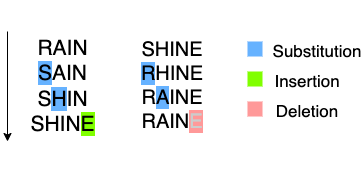
\includegraphics[width=8cm,height=3.5cm]{chapters/figures/Leven.png}
    \caption{Example showing Levenshtein distance calculation}
    \label{fig:Levenshtein}
\end{figure}

We use the Python Fuzzy-Wuzzy\footnote{https://pypi.org/project/fuzzywuzzy/} library which uses Levenshtein distance to calculate the similarity between two strings. 

We calculate the Levenshtein distance between the tokenized keywords $KW_{Q}$ in the question and the list of relations $\mathcal{R}_{DB}$ obtained from Section \ref{sec:relationsfromdbpedia}. 
The top-k candidate relations are retrieved using the following method: 
\begin{enumerate}
    \item We split the relations in $\mathcal{R}_{DB}$ into tokens as some relations in DBpedia are a sequence of concatenated tokens, as shown in Table \ref{tab:relations}.
    \item We extract the keywords in the question $KW_{Q}$ using the techniques in Section \ref{sec:preprocessnlq}. Finally, the Levenshtein distance between each keyword and the tokens in the KG relations are calculated.
    \item We retrieve the top-k relations based on the minimum distance calculated.
\end{enumerate}

\begin{table}[H]
    \centering
    \begin{tabular}{|c|c|}
     \hline
     \textbf{Relations from DBpedia} & \textbf{Split Relations} \\
    \hline
     foundedBy & founded By \\
    \hline
    associatedMusicalArtist & associated Musical Artist \\
    \hline
    foundingYear & founding Year \\
    \hline
    \end{tabular}
    \caption{Relations in DBpedia}
    \label{tab:relations}
\end{table}

\textbf{Jaro Similarity}. The Jaro distance is a measure of edit distance between two strings. Jaro Similarity is the inverse of the Jaro distance. Jaro Similarity compares two strings and gives a score representing how similar they are. It counts the characters that match between the two strings irrespective of the location, provided they are close to each other.

The Jaro similarity sim\_{j(a,b)} of two given strings a and b is give by

\begin{singlespace}
\begin{equation}
   sim_{j(a,b)} = \left\{ \begin{array}{cl}
0 & \ if \ m = 0 \\
\frac{1}{3} \left(  \frac{m}{|a|}+\frac{m}{|b|}+\frac{m-t}{m}\right)& otherwise
\end{array} \right. 
\end{equation}
\end{singlespace}

\begin{quote}
Where, \\
$|a|$ is the length of string a, \\
$|b|$ is the length of string b, \\
m is the number of similar characters, \\
t is the half the number of transpositions.
\end{quote}
Transpositions is defined as the number of matching characters
that are in a different order, divided by 2, provided they are not $\left\lfloor \frac{max(|a|,|b|)}{2} \right\rfloor - 1$ positions apart.

If two strings have completely different characters, then \textit{m = 0} and \textit{$sim_{j(a,b)} = 0$}.
If two strings are exactly the same, then 
\textit{m = $|a|$ = $|b|$} and \textit{t = 0}, hence, \textit{$sim_{j(a,b)} = 1$}.

The Jaro distance is given by,
\begin{equation}
    dist_{j}=1-sim_{j}
\end{equation}

Let us consider the strings, a=RAIN (length=4) and b=SHINE (length=5), "I" and "N" appear in both strings and in the same order, thus, no transpositions are needed. Therefore, m=2 and t=0. 
The calculation of Jaro similarity of strings a and b is shown below 
% \begin{figure}
%     \centering
%   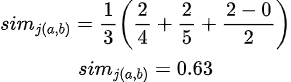
\includegraphics[width=4cm,height=1.5cm]{chapters/figures/jaro.png}
%     \caption{Example showing Jaro similarity calculation}
%     \label{fig:Levenshtein}
% \end{figure}
\begin{quote}
\centering
$sim_{j(a,b)}=\frac{1}{3} \left(  \frac{2}{4}+\frac{2}{5}+\frac{2-0}{2}\right)$ \\
$sim_{j(a,b)}=0.63$
\end{quote}

\textit{Jaro-Winkler similarity} is a modified form of Jaro similarity that increases the score by a constant if the first characters of both strings are the same. 

\begin{singlespace}
\begin{equation}
   sim_{jw(a,b)} = sim_{jw(a,b)} + lp(1-sim_{j(a,b)})
\end{equation}
\end{singlespace}

\begin{quote}
Where, \\
$sim_{j(a,b)}$ is the Jaro similarity of strings a and b, \\
$l$  is the length of common prefix at the start of the string up to a maximum of 4 characters, \\
$p$ is a constant scaling factor for how much the score is adjusted upwards for having common prefixes. The standard value for this constant is 0.1
\end{quote}

The Jaro-Winkler distance is given by,
\begin{equation}
    dist_{jw}=1-sim_{jw}
\end{equation}

If there are no common prefixes the Jaro similarity and the Jaro-Winkler similarity return the same similarity score.

We use the Python Jaro-Winkler\footnote{https://pypi.org/project/jaro-winkler/} library to calculate the Jaro similarity and the Jaro-Winkler similarity  between two strings. 

We calculate the Jaro similarity between the tokenized keywords $KW_{Q}$ in the question and the list of relations $\mathcal{R}_{DB}$ obtained from Section \ref{sec:relationsfromdbpedia}. 
The top-k candidate relations are retrieved using the following method: 
\begin{enumerate}
    \item We split the relations in $\mathcal{R}_{DB}$ into tokens as some relations in DBpedia are a sequence of concatenated tokens, as shown in Table \ref{tab:relations}.
    \item We extract the keywords in the question $KW_{Q}$ using the techniques in Section \ref{sec:preprocessnlq}. Finally, the Jaro similarity and the Jaro-Winkler similarity between each keyword and the tokens in the KG relations are calculated.
    \item We retrieve the top-k relations based on the similarity score.
\end{enumerate}

The similarity score is between \textbf{0} and \textbf{1}, where 0 means the strings are entirely different and
1 means they match exactly.

\subsection{Word Embeddings}
\label{sec:wordembeddings}
Word embedding techniques such as Word2vec\cite{word2vec}, FastText\cite{fasttext} and Glove\cite{glove} learn a numerical representation for words such that words that have the same meaning have a similar representation. Embeddings are dense vectors of floating point values which are trainable parameters. The weights are learnt by the model during training. Word embeddings are created by training a collection of fixed-length, dense and continuous-valued vectors on a huge corpus of text. A higher dimensional embedding can capture fine-grained relationships between words, but takes more data to learn. Each word in a word-embedding is represented by a point in the embedding space, which is learnt and moved based on the surrounding words. Word vectors are constructed based on the distance between each vector in the vector space. 

Contextual representations of language are functions that leverage the idea that the meaning of a particular word in a particular text depends not only on the identity of a word, but also on the words that surround it at that moment. The most popular Contextualized (Dynamic) Word Embedding techniques are BERT\cite{bert}, ElMo\cite{elmo} etc.

We analyzed two word-embedding techniques on the relations obtained from DBpedia: Word2vec and BERT.

\textbf{Word2vec.} Word2vec is one of the most popular word embedding techniques used in natural language processing. It is a feed-forward neural network with just one hidden layer. Hence, it is referred to as a Shallow Neural Network architecture. Pre-trained Word Embeddings capture the semantic and syntactic meaning of a word as they are trained on large datasets. The pre-trained Google Word2vec\footnote{https://code.google.com/archive/p/Word2vec/} model is trained on Google news data (about 100 billion words), it contains 3 million words and phrases and is fit using 300-dimensional word vectors. We use the pre-trained Word2vec model for our evaluation.

Word2vec model computes the word vector for a single token. When a token is converted to its vector representation in Word2vec, we check if that token is present in the Word2vec vocabulary. Tokens that are not present in the vocabulary (out-of-vocabulary words) are \textbf{not considered}. As some relations in DBpedia are a sequence of concatenated tokens, as shown in Table \ref{tab:relations}, we calculate the mean value of the vectors of the tokens to represent the relation as a single vector.

Consider an example relation, \textbf{associatedMusicalArtist}. The relation is an out-of-vocabulary word in the Word2vec model. We first spilt the relation into the following tokens, \textbf{associated}, \textbf{musical}, \textbf{artist}. We then convert the tokens to their corresponding vectors v1, v2 and v3 respectively and calculate the mean of the vectors. The mean of the vectors is given by
\begin{equation}
    m(n) = \frac{ v(1) + v(2) + ... + v(n)}{n}
\end{equation}
where, n is the number of tokens.

To find the similarity between the strings, we compute the cosine similarity, which is given by the dot product of the  vectors of the strings $\mathcal{A}$ and $\mathcal{B}$. The cosine similarity is given as follows,
\begin{equation}
    cosine_{sim}(\mathcal{A},\mathcal{B}) = \frac{\mathcal{A} \cdot \mathcal{B}}{||\mathcal{A}||\ ||\mathcal{B}||}
\end{equation}
where, $\mathcal{A}$ and $\mathcal{B}$ are the vectors of the strings, and $||\mathcal{A}||$ and $||\mathcal{B}||$ are the length of the two vectors $\mathcal{A}$ and $\mathcal{B}$

The top-k candidate relations are retrieved using the following method: 
\begin{enumerate}
    \item We split the relations in $\mathcal{R}_{DB}$ into tokens. Each of these tokens are converted into their corresponding vector representation and the mean of these vectors is calculated.
    \item  We extract the keywords in the question $KW_{Q}$ using the techniques in Section \ref{sec:preprocessnlq}. Each of these keywords are converted into their corresponding vector representation.
    \item Finally, the cosine similarity between each keyword and the mean vector that represents each relation in the KG relations $\mathcal{R}_{DB}$ are calculated. 
    \item We retrieve the top-k relations based on the cosine similarity score calculated.
\end{enumerate}

\textbf{BERT Embeddings.} BERT or Bidirectional Encoder Representation from Transformers, is a natural language processing pre-training developed by Google. BERT uses transformer architecture to learn embeddings for words. It is designed to pre-train deep bidirectional representations from unlabeled text including Wikipedia and Book corpus by jointly conditioning on both left and right context in all layers. BERT offers an advantage over models like Word2Vec as BERT produces word representations that are dynamically informed by the words around them while in Word2Vec each word has a fixed representation of the context within which the word appears.

We implement the BERT embedding technique using the sentence-transformers library from Python which uses HuggingFace\footnote{https://huggingface.co/sentence-transformers/bert-base-nli-mean-tokens} transformers. We use the pre-trained \textit{bert-base-nli-mean-tokens} model has 12 layers (transformer blocks), 12 attention heads, 110 million parameters and a hidden size of 768. We have approximately 54,000 relations from DBpedia. We get 54,000 embeddings each containing 768 values.

The top-k candidate relations are retrieved using the following method: 
\begin{enumerate}
    \item We split the relations in $\mathcal{R}_{DB}$ into tokens. The split tokens are encoded to get their corresponding embeddings.
    \item  We extract the keywords in the question $KW_{Q}$ using the techniques in Section \ref{sec:preprocessnlq}. Each of these keywords are encoded to obtain their corresponding embeddings.
    \item Finally, the cosine similarity between each encoded keyword and encoded tokens that represents each relation in the KG relations $\mathcal{R}_{DB}$ are calculated. 
    \item We retrieve the top-k relations based on the cosine similarity score calculated.
\end{enumerate}

The resulting similarity ranges from $-1$ to 1, where 1 means exactly the same, 0 means less similar and in-between values indicate intermediate similarity or dissimilarity.

\subsection{Term Frequency-Inverse Document Frequency}
\label{sec:tfidf}
Term Frequency - Inverse Document Frequency (TF-IDF) has the underlying concept that if a term (keyword) occurs more than once in a document, then that word is significant for that document. Also, if a term (keyword) occurs a number of times in many documents, then that term (keyword) is insignificant. The score produced by TF-IDF is based on considering the above two ideas of the frequency of occurrence of a term (keyword). 

\textbf{Term Frequency.} Term Frequency of a keyword in a document is the raw count of the keywords that appear in a document. We calculate the term frequency of a keyword using the $List_{r}$ (document) obtained in Section \ref{sec:TextCleaningPipeline}, Algorithm \ref{alg:dictcreation} (line 7).
\begin{equation}
Term \ Frequency, \ TF_{r} = \frac{count \ of \ keyword \ in \ List_{r}}{number \ of \ keywords \ in \ List_{r}}
\end{equation}
\textbf{Inverse Document Frequency.}
Inverse document frequency is used to find how common a keyword is amongst all the documents. To calculate the Document Frequency (DF) for all the keywords present in the $List_{r}$ (document) for each relation, we create a hashmap, whose key is the keyword present across all the $List_{r}$ (documents) and the value is the count of $List_{r}$ (documents) where the keyword occurs.

The Document Frequency, $DF_{keyword}$ and Inverse-Document Frequency, $IDF_{keyword}$ is given as follows
\begin{equation}
   DF_{keyword} = occurrences \ of \ keyword \ in \ N \ keyword\_List_{r}
\end{equation}
\begin{equation}
      IDF_{keyword} = log\left( \frac{N}{(DF+1)} \right)
\end{equation}
where, r is a relation in $\mathcal{R}_{DB}$ and  N is the total number of relations present in $\mathcal{R}_{DB}$. We use the logarathmic inverse while calculating IDF as the N value is large such that it dampens the importance of term that has a high frequency. 

The TF-IDF for a relation r and a keyword is a hashmap, whose key is relation-keyword pair and the value is the TF-IDF score, which is given by
\begin{equation}
      TF-IDF \ [r,keyword] = TF_{r}*IDF_{keyword}
\end{equation}

The top-k candidate relations are retrieved using the following method: 
\begin{enumerate}
    \item  We extract the keywords in the question $KW_{Q}$ using the techniques in Section \ref{sec:preprocessnlq}. Each of these keywords are searched in the key of the TF-IDF hashmap.
    \item We retrieve the top-k relations based on TF-IDF scores returned for each keyword.
    % \item Finally, the cosine similarity between each keyword and the mean vector that represent each relation in the KG relations $\mathcal{R}_{DB}$ are calculated. 
    % \item We retrieve the top-k relations based on the cosine similarity score calculated.
\end{enumerate}
Let us consider an example keyword "bear" (lemmatized form of born), we check in every document if this keyword exists and if the keyword exists, then the TF-IDF value is returned for that particular relation (the document where it occurs). We sort the TF-IDF scores and display the top k relations. The top-5 relations returned for the keyword "bear" are \textit{cityOfBirth, nationality(ethnicOrigin), yearOfBirth, countryOfBirth} and \textit{originally}.

\section{Results}
In this section, we discuss the results from the experiments over our datasets and baselines.

We first evaluate the Hits@k (k=5, 10, 15) results of ReMLOFT and the other baselines. We compare the performance of our system with 5 other techniques, Levenshtein distance, Jaro similarity, Jaro-Winkler similarity, Word2vec, BERT and TF-IDF. Figure \ref{fig:top5hits} shows the Hits@5, Figure \ref{fig:top10hits} shows the Hits@10 and Figure \ref{fig:top15hits} shows the Hits@15 for the QALD datasets across all the baselines. We notice that the Hits@k increases significantly when k is increased across all the datasets. 
As the complexity of the question increases, the number of expected relations to build a SPARQL query increases. 
Increase in k in ReMLOFT yeilds better results due to the noisy nature of the information-dense free-text knowledge graph.


\begin{figure}[p]
    \centering
    \begin{minipage}{0.7\textwidth}
   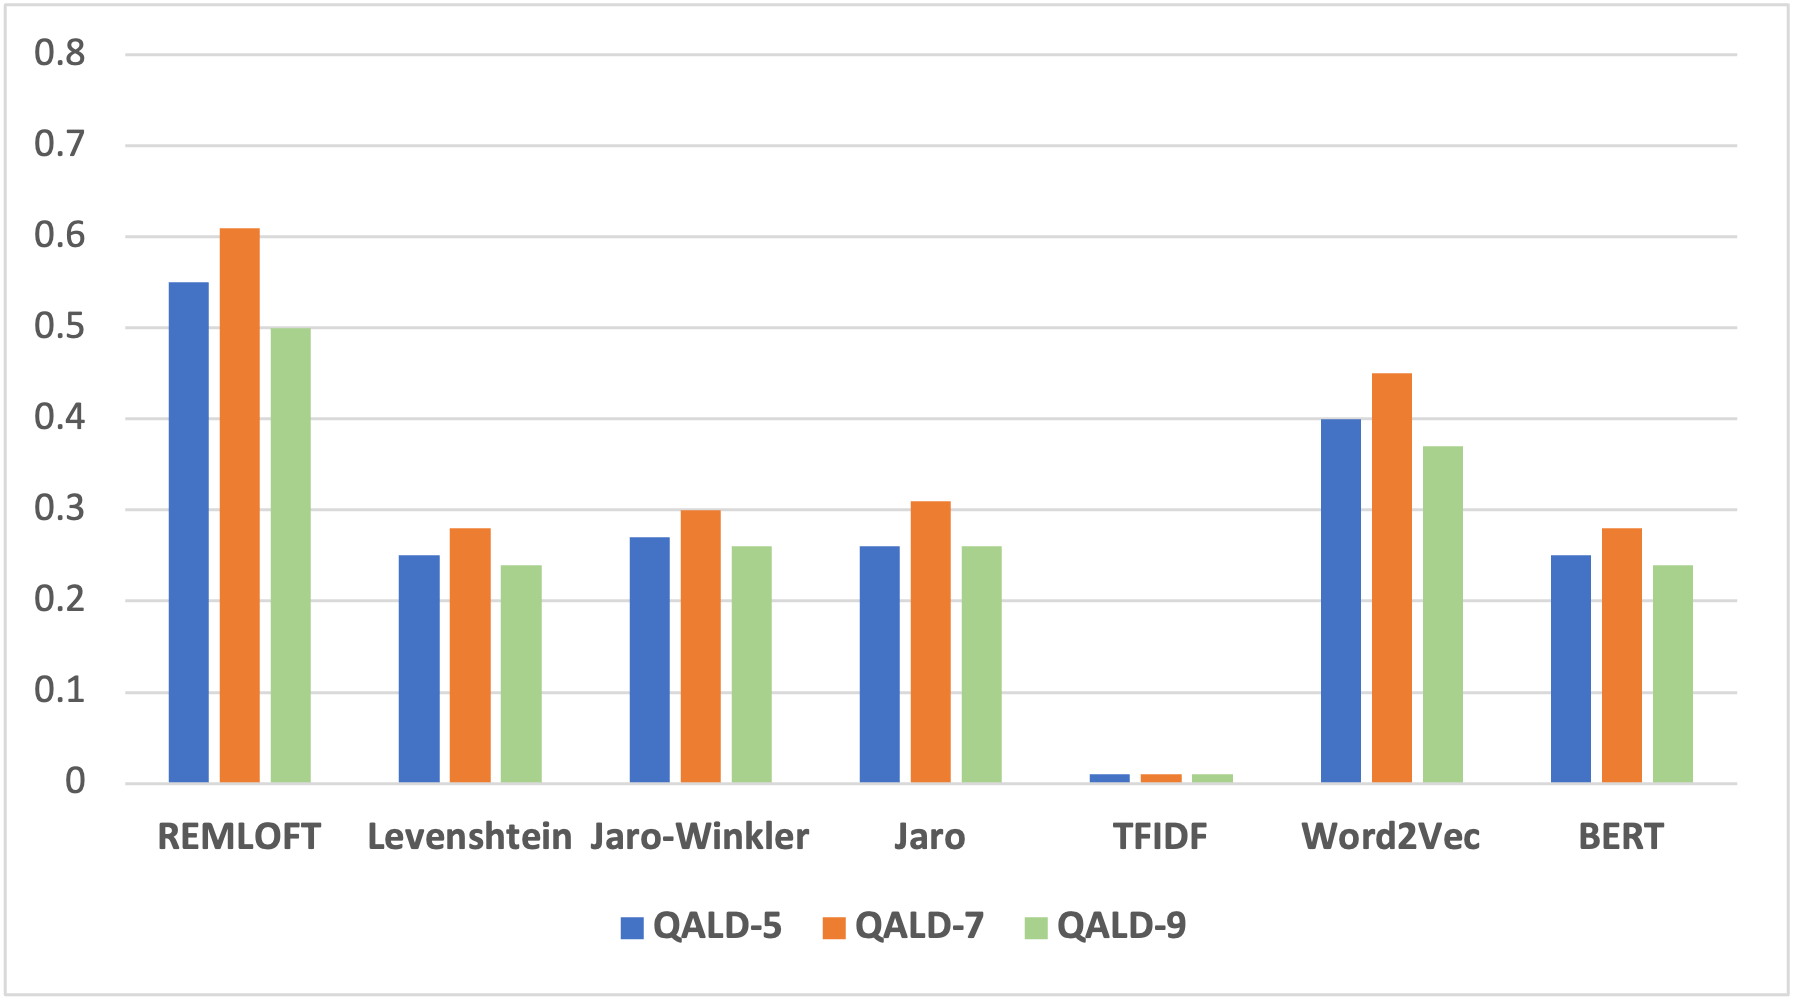
\includegraphics[width=\textwidth]{chapters/figures/top5bert.png}
    \caption{Hits@5 ReMLOFT vs other baselines}
    \label{fig:top5hits}
     \end{minipage}
         \begin{minipage}{0.7\textwidth}
   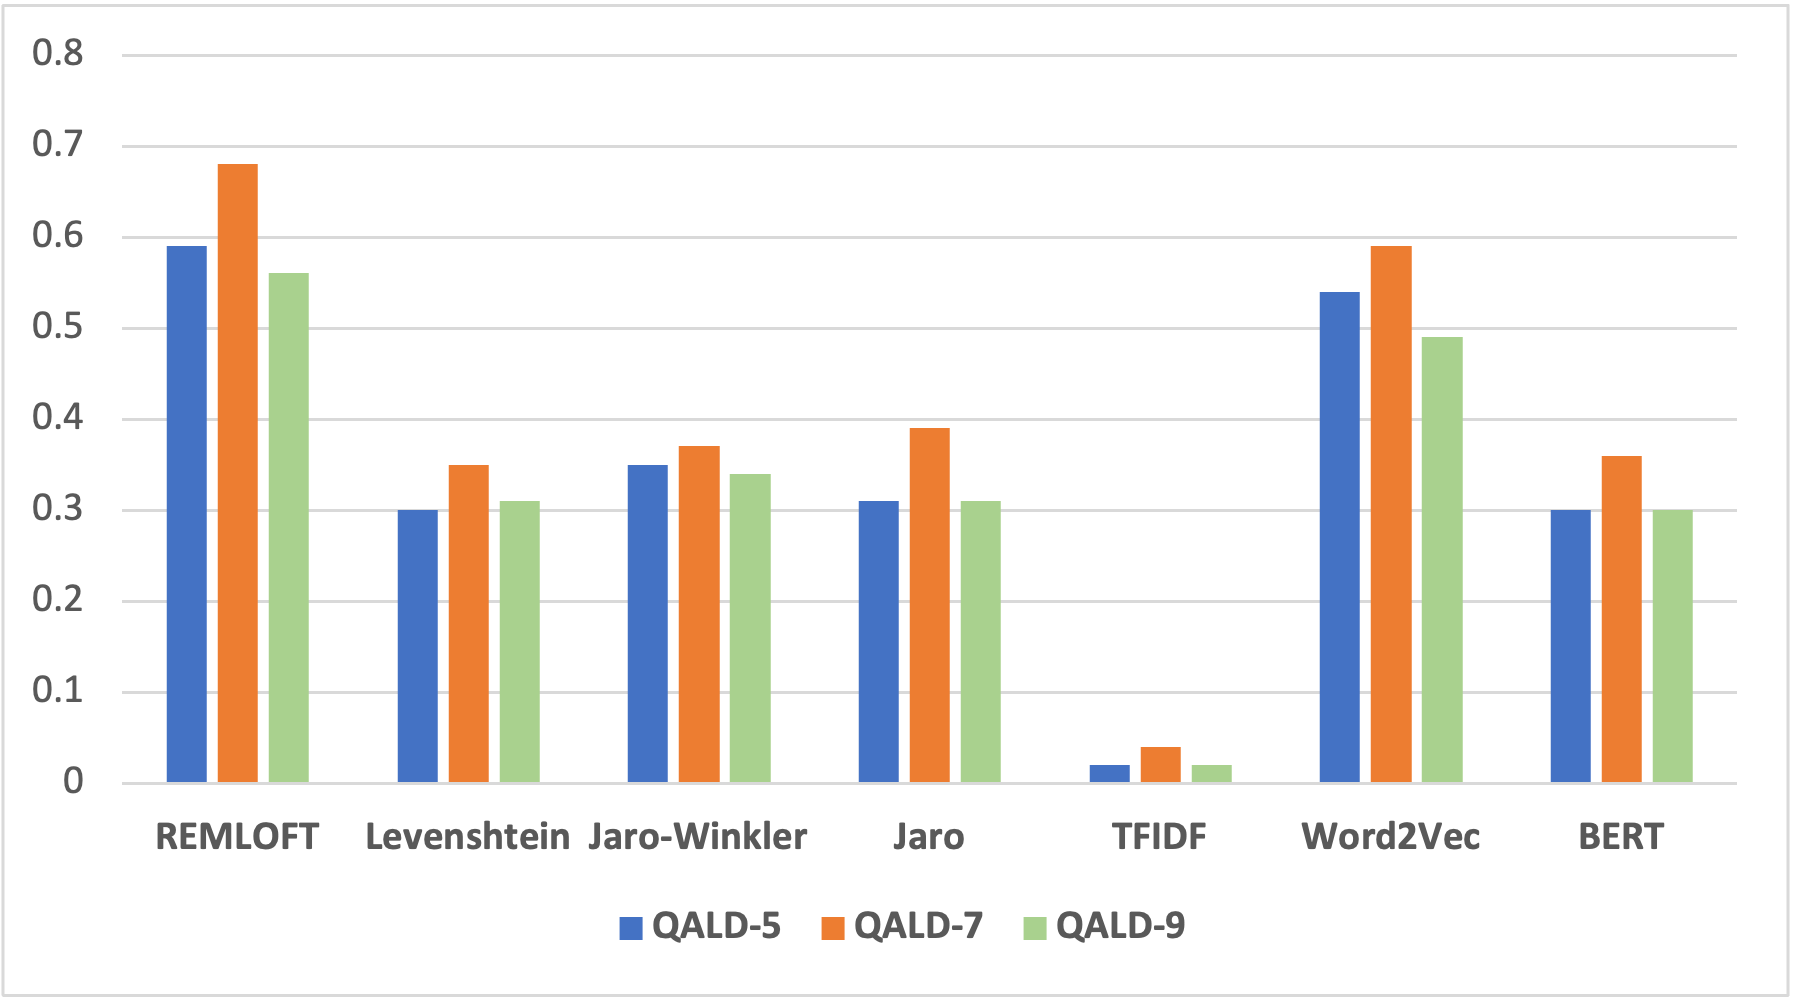
\includegraphics[width=\textwidth]{chapters/figures/top10bert.png}
    \caption{Hits@10 ReMLOFT vs other baselines}
    \label{fig:top10hits}
     \end{minipage}
         \begin{minipage}{0.7\textwidth}
    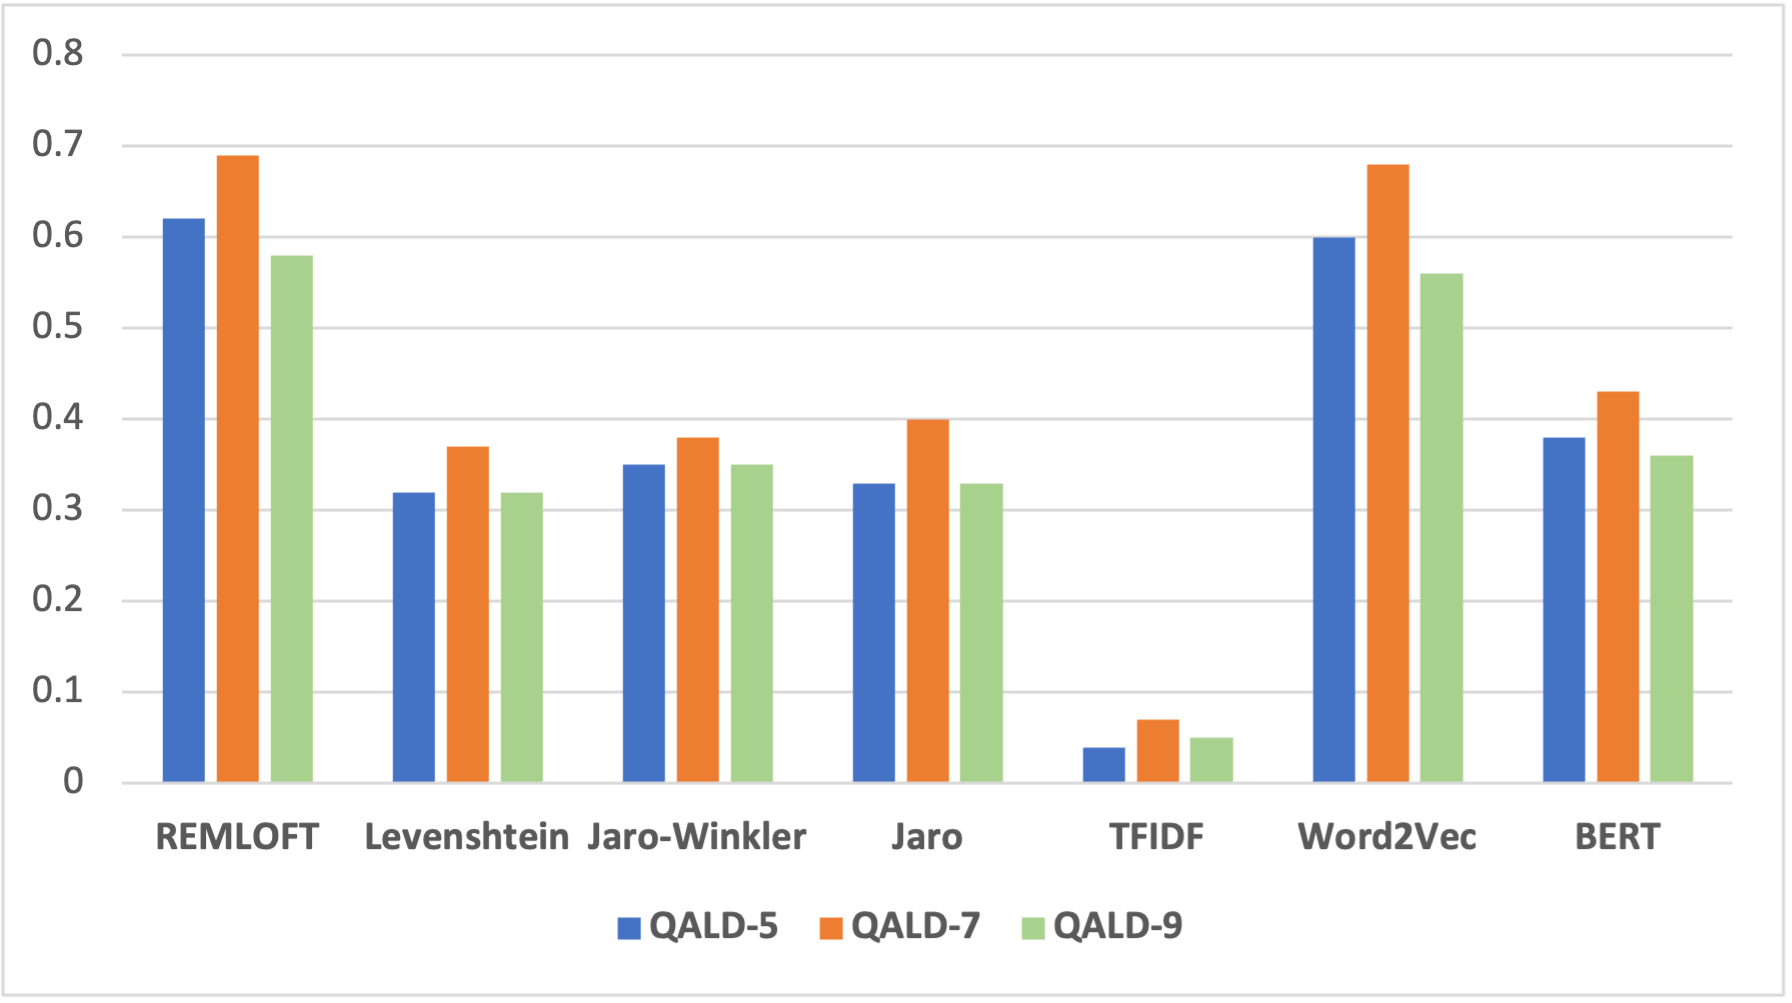
\includegraphics[width=\textwidth]{chapters/figures/Top15Bert.png}
        \caption{Hits@15 ReMLOFT vs other baselines}
        \label{fig:top15hits}
    \end{minipage}
\end{figure}


Both string similarity and word embedding methods are used on the list of relations $\mathcal{R}_{DB}$. Though string similarity is practical for words with spelling errors or plural forms of words, they do not capture the semantics of the keyword. String similarity techniques are successful for questions such as \textit{Who developed Slack?}, expected relation: \textit{developer}, where the keyword \textit{develop} is used for the search,
but \textbf{fail} to answer questions like \textit{Who is the host of the BBC Wildlife Specials?} where the expected relation: \textit{presenter} cannot be matched with the keyword \textit{host}. 

To overcome the limitation of the string similarity techniques used, we use the pre-trained word embeddings from Word2vec. We observe a significant increase in the Hits@k value. This is because word embeddings capture the semantics of the relations, thereby returning semantically similar relations. Word2vec represents every word as an independent vector and thus we compute the mean of the word vectors to receive a single vector. Averaging of vector representations using pre-trained word embeddings results in the loss of information. The pre-trained word embedding approach has the constraint of out-of-vocabulary words. Some of the tokens mentioned in the relations are not found in the Word2Vec vocabulary. When the model encounters a new word, it skips the word, thereby making it less ideal to capture the similarity of the keyword. Though word-embeddings give satisfactory results, they cannot be extended to other domains unless the word embedding is trained using specific domain vocabulary.

Word-level similarity comparisons are not appropriate with BERT embeddings because these embeddings are contextually dependent, meaning that the word vector changes depending on the sentence it appears in. Contextually dependent vectors can be obtained only in the sentence-level and not in the word-level similarity. Since we compare each keyword in the question with the relations from DBpedia, BERT doesn't give exceptional results. 

We also evaluate the TF-IDF on the free-text KG. We observe that the TF-IDF method performs unsatisfactorily as compared to the other methods used. This is due to the large frequency of certain words in the relation documents. For a given keyword k, if we consider there are 10,000 documents that contain the keyword and 1000 documents that do not contain the keyword, the inverse document frequency of k is very low (because it is found in almost all documents), and k gets a very small TF-IDF score. The same argument applies for TF, given 2 documents - one consisting of 100 unique words, and the other of 1000 unique words, each word in the first document will have a TF of 0.01 while in document 2 each word will have a TF of 0.001 which casues the TF for each document to have a large bias.

\begin{table}[H]
    \centering
    \begin{tabular}{|c|c|c|c|c|}
     \hline
     \textbf{No of Relations} & \textbf{QALD-5} & \textbf{QALD-7} & \textbf{QALD-9}  \\
    \hline
     1 Relation & 0.65 & 0.71	& 0.61 \\
    \hline
    2 Relations & 0.83 & 0.83 & 0.80 \\
    \hline
    3 Relations & 0.63 & 1	& 0.83 \\
    \hline
    4 Relations & 1 & - & 0 \\
    \hline
        Total Coverage & 0.69 & 0.74 & 0.65 \\
            \hline
    \end{tabular}
    \caption{ReMLOFT Coverage for Questions based on the number of relations}
    \label{tab:relationcoverage}
\end{table}

We then evaluate the Coverage of ReMLOFT for the QALD datasets as shown in Table \ref{tab:relationcoverage}. ReMLOFT performs exceptionally for complex questions with more than one relation and has adequate coverage for simple questions. We see that ReMLOFT performs well for questions with two relations across all the datasets with nearly \textbf{80\%} coverage. 
\begin{figure}[h]
    \centering
   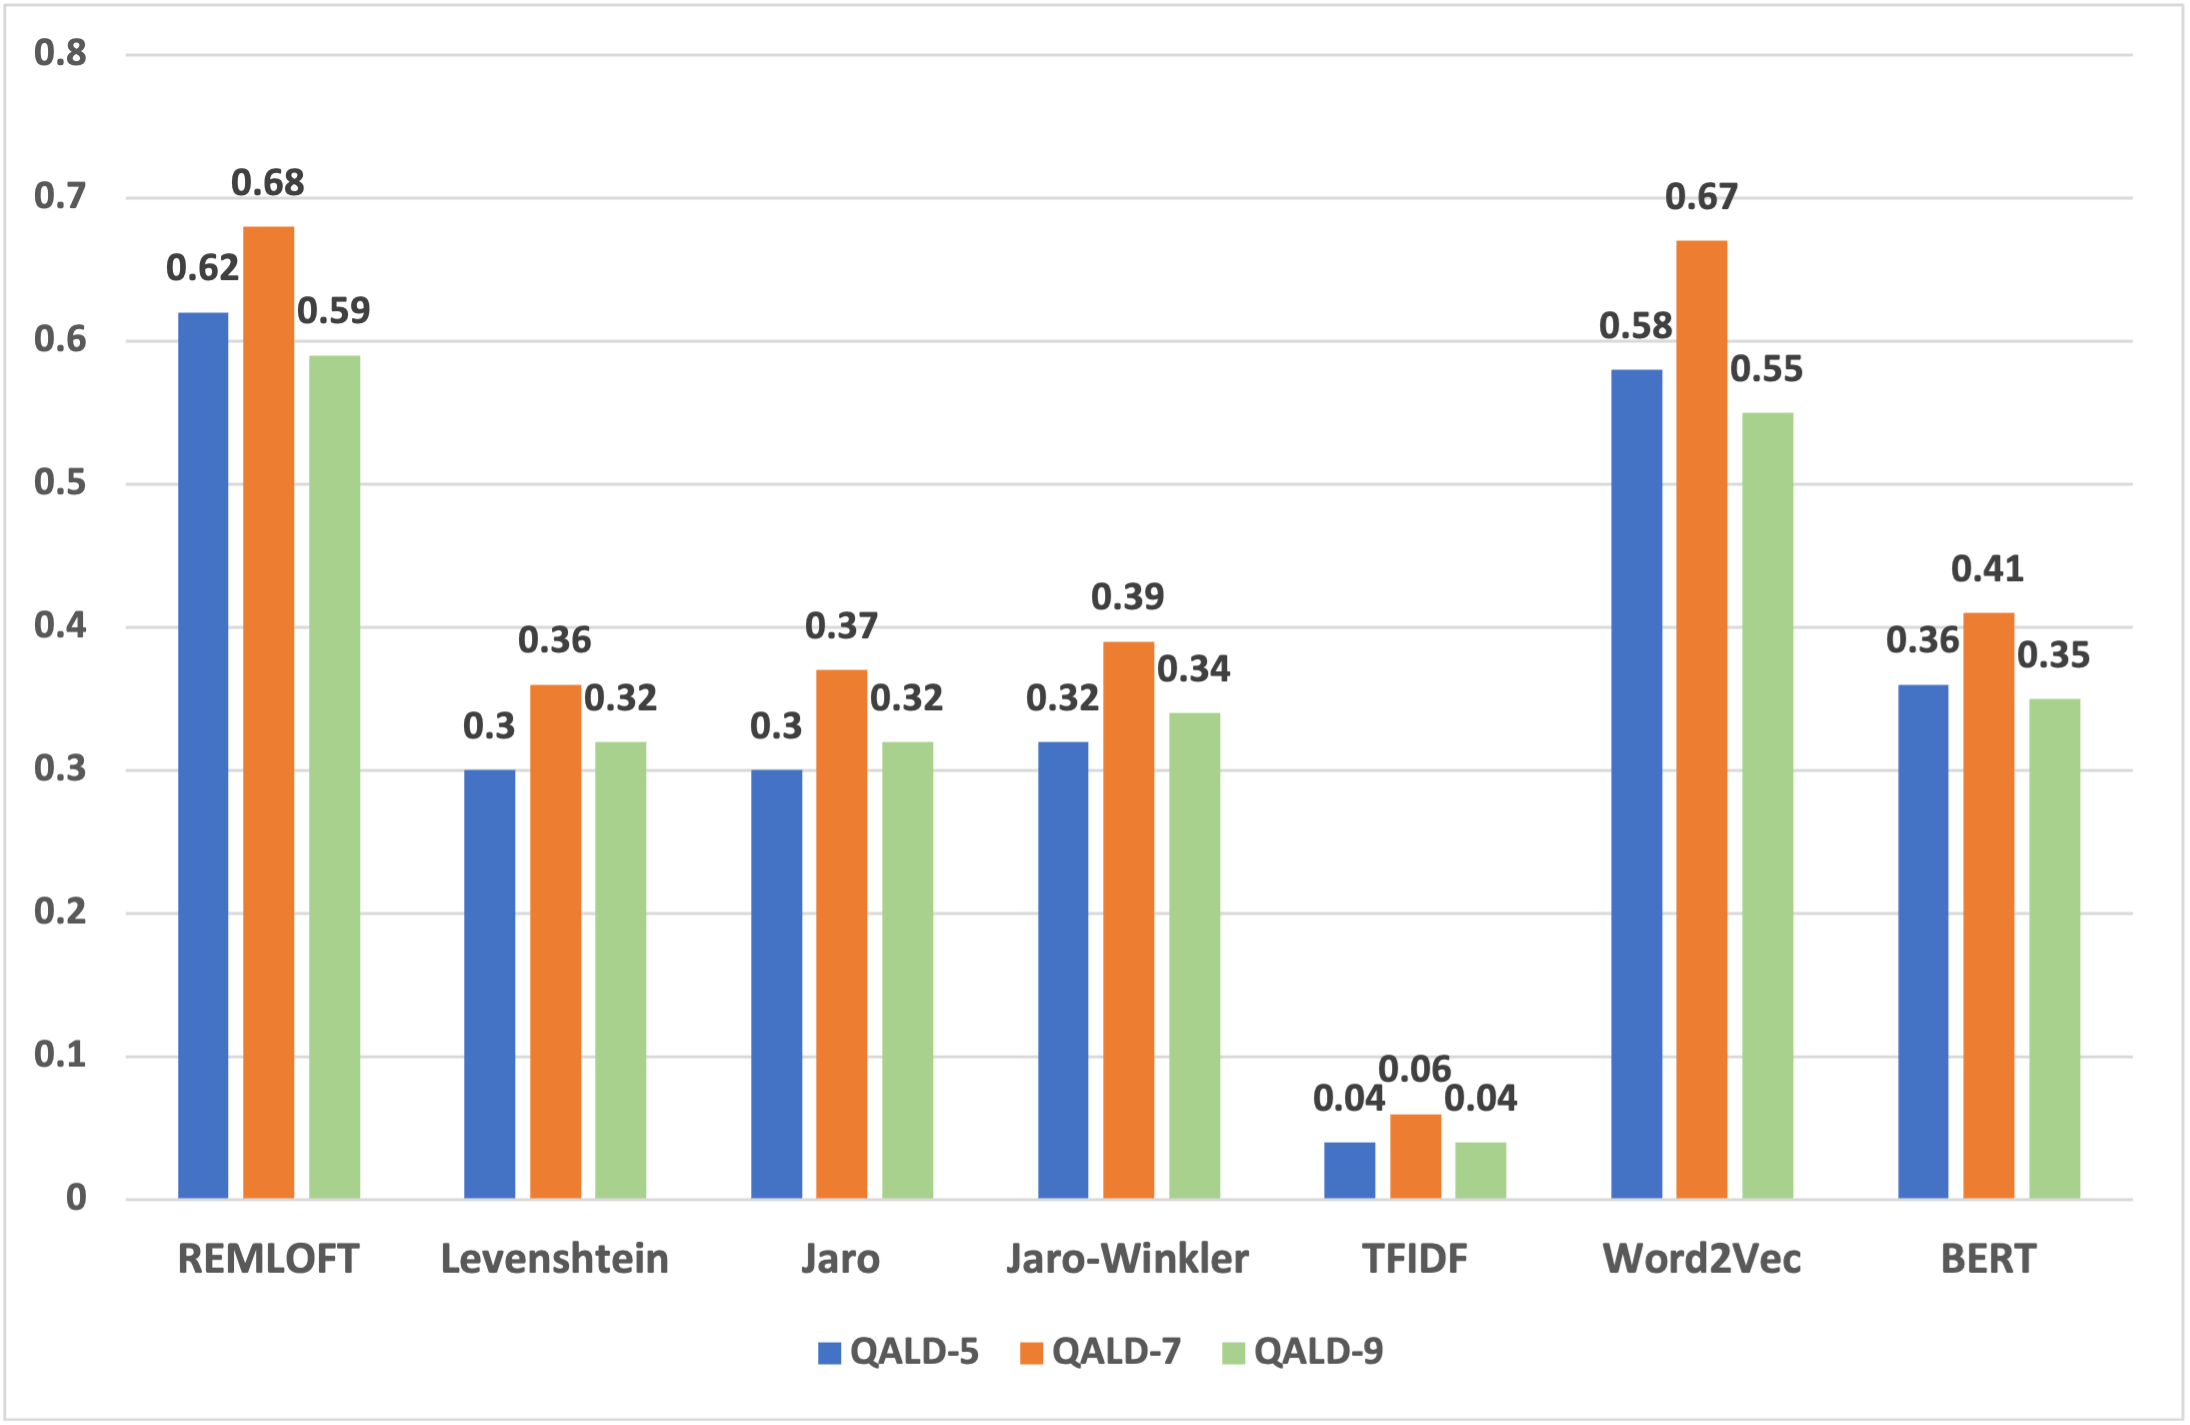
\includegraphics[width=10cm, height=6cm]{chapters/figures/accuracyBert.png}
    \caption{Accuracy of ReMLOFT vs other baselines}
    \label{fig:graphacc}
\end{figure}

We evaluate the accuracy of ReMLOFT in comparison with the other baselines. We observe that the accuracy of ReMLOFT varies based on the number of questions in the dataset. ReMLOFT returns 163 relations from a total of 262 relations for QALD-5, 142 relations from a total of 209 relations for QALD-7 and 259 relations from a total of 441 relations for QALD-9. Figure \ref{fig:graphacc} shows that ReMLOFT represents a vast improvement in accuracy when compared to the baselines.

In conclusion, ReMLOFT performs better than the baseline techniques to map relations, especially for questions with multiple expected relations. 

\section{Limitations}
In this section, we investigate the shortcomings of our approach.

\textbf{Missing Entity.} Some questions found in the QALD dataset do not have an entity. For example, {\fontfamily{pcr}\selectfont Which countries have more than two official languages?}, has no given entity. Our approach relies on the relations returned by DBpedia entities to reduce the the number of candidate relations. Therefore, questions without an entity don't return a result even though the keywords from the question return valid relations from the Free-text KG. The candidate relations from the Free-text KG is a large search space. Hence, pruning the necessary candidate relations would require extensive filtering. 

\textbf{Insufficient Keywords.} ReMLOFT does not work effectively if there are not enough keywords in the question that describes the context of the question. 
Consider the following example questions below,
\begin{enumerate}
    \item \textbf{Where in France is sparkling wine produced?}, has two gold standard entities, \textit{"sparkling wine"} and \textit{"France"}. However, the keyword \textbf{produce}, is not sufficient to return the expected relations \textit{wineProduced} and \textit{location}. 
    \item \textbf{Was Margaret Thatcher a chemist?}, with the gold standard entities \textit{"Margaret Thatcher"} and \textit{"chemist"}. We are left with \textit{no keywords} to evaluate the question.
\end{enumerate}

Including the entities as keywords for mapping relations from the free-text KG could overcome this problem, but this would introduce a lot of noise and increase the number of candidate relations to filter from.

\textbf{Semantic Significance.} Though our approach captures the semantics of a specific word using the knowledge from the Free-text KG. It does not always imply the top ranking of the correct relations for certain keywords. A keyword could be closely related to another relation than the expected gold standard relations.
Consider the question, \textbf{How much did Pulp Fiction cost?}, where the expected gold standard relation is \textit{budget}. The keyword \textbf{cost} maps to the relations \textbf{cost} and \textbf{netIncome} as the top two relations from the free-text KG.

\textbf{Effect of n-grams.} Since our approach uses unigrams, keywords that are n-grams do not work effectively. A keyword \textbf{timezone} returns less significant relations as compared to \textbf{time zone} which returns the expected gold standard relation.


\chapter{Conclusion and Future Work}
In this thesis, we present an interactive relation mapping approach, ReMLOFT, for answering simple and complex questions, by leveraging an information-dense free-text knowledge graph. We also investigate the utilization of the free-text knowledge graph to find out which keywords are semantically similar to the ones in the question by creating a dictionary of the most frequent keywords using example sentences from Wikipedia. While keeping the model simple by refraining from using highly complicated machine learning models and neural networks, our approach achieves competitive results when compared to the baselines. 

In comparison to other relation mapping approaches \cite{falcon, falcon2, kbpearl}, we explore the relation mapping problem as an interactive method by exploiting richer word-level semantics than those captured by string similarity or word embedding techniques. Our approach gives the user the pliability to investigate various options to build better SPARQL queries for question answering systems. In addition, our approach could be integrated with existing query completion and query assisting tools to enhance the capability of their systems.

We believe our model is easily transferable to various knowledge graphs across multiple domains and is acceptable for frequently evolving KGs, as our approach does not learn KG-specific representations. 

In future, we aim to focus on better candidate pruning and noise reduction to improve the learning of relation patterns. We further plan to extend the assessment of the portability of our model across various domains and knowledge graphs. Our approach will be fine-tuned to produce more compelling outcomes, allowing for a more comprehensive quantitative comparison.

\end{document}
